\documentclass[twoside]{book}

% Packages required by doxygen
\usepackage{calc}
\usepackage{doxygen}
\usepackage{graphicx}
\usepackage[utf8]{inputenc}
\usepackage{makeidx}
\usepackage{multicol}
\usepackage{multirow}
\usepackage{textcomp}
\usepackage[table]{xcolor}

% Font selection
\usepackage[T1]{fontenc}
\usepackage{mathptmx}
\usepackage[scaled=.90]{helvet}
\usepackage{courier}
\usepackage{amssymb}
\usepackage{sectsty}
\renewcommand{\familydefault}{\sfdefault}
\allsectionsfont{%
  \fontseries{bc}\selectfont%
  \color{darkgray}%
}
\renewcommand{\DoxyLabelFont}{%
  \fontseries{bc}\selectfont%
  \color{darkgray}%
}

% Page & text layout
\usepackage{geometry}
\geometry{%
  a4paper,%
  top=2.5cm,%
  bottom=2.5cm,%
  left=2.5cm,%
  right=2.5cm%
}
\tolerance=750
\hfuzz=15pt
\hbadness=750
\setlength{\emergencystretch}{15pt}
\setlength{\parindent}{0cm}
\setlength{\parskip}{0.2cm}
\makeatletter
\renewcommand{\paragraph}{%
  \@startsection{paragraph}{4}{0ex}{-1.0ex}{1.0ex}{%
    \normalfont\normalsize\bfseries\SS@parafont%
  }%
}
\renewcommand{\subparagraph}{%
  \@startsection{subparagraph}{5}{0ex}{-1.0ex}{1.0ex}{%
    \normalfont\normalsize\bfseries\SS@subparafont%
  }%
}
\makeatother

% Headers & footers
\usepackage{fancyhdr}
\pagestyle{fancyplain}
\fancyhead[LE]{\fancyplain{}{\bfseries\thepage}}
\fancyhead[CE]{\fancyplain{}{}}
\fancyhead[RE]{\fancyplain{}{\bfseries\leftmark}}
\fancyhead[LO]{\fancyplain{}{\bfseries\rightmark}}
\fancyhead[CO]{\fancyplain{}{}}
\fancyhead[RO]{\fancyplain{}{\bfseries\thepage}}
\fancyfoot[LE]{\fancyplain{}{}}
\fancyfoot[CE]{\fancyplain{}{}}
\fancyfoot[RE]{\fancyplain{}{\bfseries\scriptsize Generated on Wed Dec 3 2014 10\-:51\-:06 for Bank by Doxygen }}
\fancyfoot[LO]{\fancyplain{}{\bfseries\scriptsize Generated on Wed Dec 3 2014 10\-:51\-:06 for Bank by Doxygen }}
\fancyfoot[CO]{\fancyplain{}{}}
\fancyfoot[RO]{\fancyplain{}{}}
\renewcommand{\footrulewidth}{0.4pt}
\renewcommand{\chaptermark}[1]{%
  \markboth{#1}{}%
}
\renewcommand{\sectionmark}[1]{%
  \markright{\thesection\ #1}%
}

% Indices & bibliography
\usepackage{natbib}
\usepackage[titles]{tocloft}
\setcounter{tocdepth}{3}
\setcounter{secnumdepth}{5}
\makeindex

% Hyperlinks (required, but should be loaded last)
\usepackage{ifpdf}
\ifpdf
  \usepackage[pdftex,pagebackref=true]{hyperref}
\else
  \usepackage[ps2pdf,pagebackref=true]{hyperref}
\fi
\hypersetup{%
  colorlinks=true,%
  linkcolor=blue,%
  citecolor=blue,%
  unicode%
}

% Custom commands
\newcommand{\clearemptydoublepage}{%
  \newpage{\pagestyle{empty}\cleardoublepage}%
}


%===== C O N T E N T S =====

\begin{document}

% Titlepage & ToC
\hypersetup{pageanchor=false}
\pagenumbering{roman}
\begin{titlepage}
\vspace*{7cm}
\begin{center}%
{\Large Bank \\[1ex]\large Assignment 1 }\\
\vspace*{1cm}
{\large Generated by Doxygen 1.8.6}\\
\vspace*{0.5cm}
{\small Wed Dec 3 2014 10:51:06}\\
\end{center}
\end{titlepage}
\clearemptydoublepage
\tableofcontents
\clearemptydoublepage
\pagenumbering{arabic}
\hypersetup{pageanchor=true}

%--- Begin generated contents ---
\chapter{Namespace Index}
\section{Namespace List}
Here is a list of all documented namespaces with brief descriptions\-:\begin{DoxyCompactList}
\item\contentsline{section}{\hyperlink{namespaceDb}{Db} \\*C++ abstraction for database implementations }{\pageref{namespaceDb}}{}
\end{DoxyCompactList}

\chapter{Hierarchical Index}
\section{Class Hierarchy}
This inheritance list is sorted roughly, but not completely, alphabetically\-:\begin{DoxyCompactList}
\item \contentsline{section}{Account}{\pageref{classAccount}}{}
\begin{DoxyCompactList}
\item \contentsline{section}{Chequing\-Account}{\pageref{classChequingAccount}}{}
\item \contentsline{section}{Credit\-Account}{\pageref{classCreditAccount}}{}
\item \contentsline{section}{Savings\-Account}{\pageref{classSavingsAccount}}{}
\end{DoxyCompactList}
\item \contentsline{section}{Account\-Table}{\pageref{classAccountTable}}{}
\item \contentsline{section}{Db\-:\-:Db}{\pageref{classDb_1_1Db}}{}
\item \contentsline{section}{Db\-:\-:db\-\_\-rows}{\pageref{structDb_1_1db__rows}}{}
\item \contentsline{section}{Fund\-Movement\-Validation}{\pageref{classFundMovementValidation}}{}
\item \contentsline{section}{Logger}{\pageref{classLogger}}{}
\item \contentsline{section}{Maintenance\-Methods}{\pageref{classMaintenanceMethods}}{}
\item \contentsline{section}{Manager\-Methods}{\pageref{classManagerMethods}}{}
\item \contentsline{section}{Payment}{\pageref{classPayment}}{}
\item \contentsline{section}{Payment\-Table}{\pageref{classPaymentTable}}{}
\item \contentsline{section}{Purchase}{\pageref{classPurchase}}{}
\item \contentsline{section}{Purchase\-Table}{\pageref{classPurchaseTable}}{}
\item \contentsline{section}{User\-:\-:User}{\pageref{classUser_1_1User}}{}
\item \contentsline{section}{User\-Methods}{\pageref{classUserMethods}}{}
\item \contentsline{section}{usermethods}{\pageref{classusermethods}}{}
\item \contentsline{section}{User\-:\-:User\-Table}{\pageref{classUser_1_1UserTable}}{}
\item \contentsline{section}{Utilities}{\pageref{classUtilities}}{}
\end{DoxyCompactList}

\chapter{Class Index}
\section{Class List}
Here are the classes, structs, unions and interfaces with brief descriptions\-:\begin{DoxyCompactList}
\item\contentsline{section}{\hyperlink{classAccount}{Account} }{\pageref{classAccount}}{}
\item\contentsline{section}{\hyperlink{classAccountTable}{Account\-Table} }{\pageref{classAccountTable}}{}
\item\contentsline{section}{\hyperlink{classChequingAccount}{Chequing\-Account} }{\pageref{classChequingAccount}}{}
\item\contentsline{section}{\hyperlink{classCreditAccount}{Credit\-Account} }{\pageref{classCreditAccount}}{}
\item\contentsline{section}{\hyperlink{classDb_1_1Db}{Db\-::\-Db} \\*C++ class wrapper for a handful of static methods for accessing databases }{\pageref{classDb_1_1Db}}{}
\item\contentsline{section}{\hyperlink{structDb_1_1db__rows}{Db\-::db\-\_\-rows} \\*A container for a set of rows }{\pageref{structDb_1_1db__rows}}{}
\item\contentsline{section}{\hyperlink{classFundMovementValidation}{Fund\-Movement\-Validation} }{\pageref{classFundMovementValidation}}{}
\item\contentsline{section}{\hyperlink{classLogger}{Logger} }{\pageref{classLogger}}{}
\item\contentsline{section}{\hyperlink{classMaintenanceMethods}{Maintenance\-Methods} }{\pageref{classMaintenanceMethods}}{}
\item\contentsline{section}{\hyperlink{classManagerMethods}{Manager\-Methods} }{\pageref{classManagerMethods}}{}
\item\contentsline{section}{\hyperlink{classPayment}{Payment} }{\pageref{classPayment}}{}
\item\contentsline{section}{\hyperlink{classPaymentTable}{Payment\-Table} }{\pageref{classPaymentTable}}{}
\item\contentsline{section}{\hyperlink{classPurchase}{Purchase} }{\pageref{classPurchase}}{}
\item\contentsline{section}{\hyperlink{classPurchaseTable}{Purchase\-Table} }{\pageref{classPurchaseTable}}{}
\item\contentsline{section}{\hyperlink{classSavingsAccount}{Savings\-Account} }{\pageref{classSavingsAccount}}{}
\item\contentsline{section}{\hyperlink{classUser_1_1User}{User\-::\-User} }{\pageref{classUser_1_1User}}{}
\item\contentsline{section}{\hyperlink{classUserMethods}{User\-Methods} }{\pageref{classUserMethods}}{}
\item\contentsline{section}{\hyperlink{classusermethods}{usermethods} }{\pageref{classusermethods}}{}
\item\contentsline{section}{\hyperlink{classUser_1_1UserTable}{User\-::\-User\-Table} \\*A list of static methods that access to the database for the \hyperlink{classUser_1_1User}{User} class }{\pageref{classUser_1_1UserTable}}{}
\item\contentsline{section}{\hyperlink{classUtilities}{Utilities} \\*A wrapper class for general, repetitive tasks }{\pageref{classUtilities}}{}
\end{DoxyCompactList}

\chapter{Namespace Documentation}
\hypertarget{namespaceDb}{\section{Db Namespace Reference}
\label{namespaceDb}\index{Db@{Db}}
}


c++ abstraction for database implementations  


\subsection*{Classes}
\begin{DoxyCompactItemize}
\item 
struct \hyperlink{structDb_1_1db__rows}{db\-\_\-rows}
\begin{DoxyCompactList}\small\item\em A container for a set of rows. \end{DoxyCompactList}\item 
class \hyperlink{classDb_1_1Db}{Db}
\begin{DoxyCompactList}\small\item\em c++ class wrapper for a handful of static methods for accessing databases \end{DoxyCompactList}\end{DoxyCompactItemize}


\subsection{Detailed Description}
c++ abstraction for database implementations Wraps around a database library and provides c++ access.

Rows vector$<$string$>$, a set of rows are vector$<$vector$<$string$>$ $>$ are vector$<$vector$<$string$>$ $>$ and column names are vector$<$string$>$

A struct called \hyperlink{structDb_1_1db__rows}{db\-\_\-rows} has been provided to take care of sets of rows but you'll have to construct single rows yourself \begin{DoxyAuthor}{Author}
james 
\end{DoxyAuthor}
\begin{DoxyDate}{Date}
September 2014 
\end{DoxyDate}

\chapter{Class Documentation}
\hypertarget{classAccount}{\section{Account Class Reference}
\label{classAccount}\index{Account@{Account}}
}


Inheritance diagram for Account\-:
\nopagebreak
\begin{figure}[H]
\begin{center}
\leavevmode
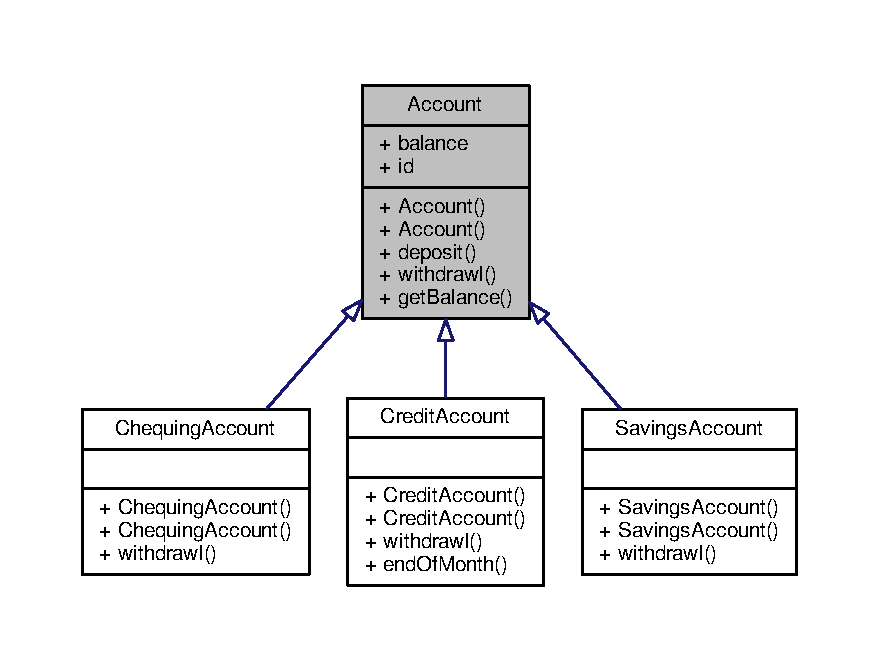
\includegraphics[width=350pt]{classAccount__inherit__graph}
\end{center}
\end{figure}


Collaboration diagram for Account\-:
\nopagebreak
\begin{figure}[H]
\begin{center}
\leavevmode
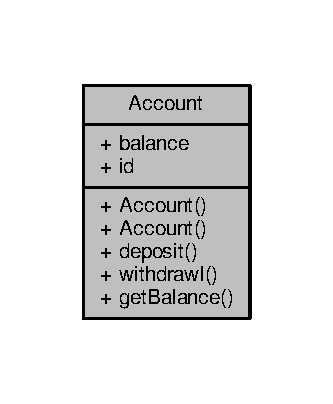
\includegraphics[width=160pt]{classAccount__coll__graph}
\end{center}
\end{figure}
\subsection*{Public Member Functions}
\begin{DoxyCompactItemize}
\item 
\hypertarget{classAccount_a366660970b5eeb5c17436062327f1b14}{\hyperlink{classAccount_a366660970b5eeb5c17436062327f1b14}{Account} ()}\label{classAccount_a366660970b5eeb5c17436062327f1b14}

\begin{DoxyCompactList}\small\item\em Empty account constructor. Sets balance and id to 0. \end{DoxyCompactList}\item 
\hyperlink{classAccount_a8aec0e7394567f9fad51e5c2ca74ba02}{Account} (double starting\-\_\-balance)
\begin{DoxyCompactList}\small\item\em constructor that sets a starting balance \end{DoxyCompactList}\item 
int \hyperlink{classAccount_a577fd69104cecb1115094f191e539e03}{deposit} (double amount)
\begin{DoxyCompactList}\small\item\em deposits money into the particular class \end{DoxyCompactList}\item 
virtual int \hyperlink{classAccount_afe06e68bfc0e09eee1d39093c8f84704}{withdrawl} (double amount)
\begin{DoxyCompactList}\small\item\em virtual withdrawl method. Accounts that inherit from \hyperlink{classAccount}{Account} must implement withdrawl \end{DoxyCompactList}\item 
double \hyperlink{classAccount_a60839724cf983feea4546148ceabcc5f}{get\-Balance} ()
\begin{DoxyCompactList}\small\item\em gets balance of the account \end{DoxyCompactList}\end{DoxyCompactItemize}
\subsection*{Public Attributes}
\begin{DoxyCompactItemize}
\item 
\hypertarget{classAccount_a6e41f403b4813738ba835377f212de33}{double {\bfseries balance}}\label{classAccount_a6e41f403b4813738ba835377f212de33}

\item 
\hypertarget{classAccount_a296dcba09b2c9e7234a6b2afd3ce0ffb}{int {\bfseries id}}\label{classAccount_a296dcba09b2c9e7234a6b2afd3ce0ffb}

\end{DoxyCompactItemize}


\subsection{Constructor \& Destructor Documentation}
\hypertarget{classAccount_a8aec0e7394567f9fad51e5c2ca74ba02}{\index{Account@{Account}!Account@{Account}}
\index{Account@{Account}!Account@{Account}}
\subsubsection[{Account}]{\setlength{\rightskip}{0pt plus 5cm}Account\-::\-Account (
\begin{DoxyParamCaption}
\item[{double}]{starting\-\_\-balance}
\end{DoxyParamCaption}
)\hspace{0.3cm}{\ttfamily [inline]}}}\label{classAccount_a8aec0e7394567f9fad51e5c2ca74ba02}


constructor that sets a starting balance 


\begin{DoxyParams}{Parameters}
{\em starting\-\_\-balance} & the amount of money to start with in an account \\
\hline
\end{DoxyParams}


\subsection{Member Function Documentation}
\hypertarget{classAccount_a577fd69104cecb1115094f191e539e03}{\index{Account@{Account}!deposit@{deposit}}
\index{deposit@{deposit}!Account@{Account}}
\subsubsection[{deposit}]{\setlength{\rightskip}{0pt plus 5cm}int Account\-::deposit (
\begin{DoxyParamCaption}
\item[{double}]{amount}
\end{DoxyParamCaption}
)}}\label{classAccount_a577fd69104cecb1115094f191e539e03}


deposits money into the particular class 


\begin{DoxyParams}{Parameters}
{\em amount} & the amount to deposit \\
\hline
\end{DoxyParams}
\begin{DoxyReturn}{Returns}
integer for success or failure 
\end{DoxyReturn}
\hypertarget{classAccount_a60839724cf983feea4546148ceabcc5f}{\index{Account@{Account}!get\-Balance@{get\-Balance}}
\index{get\-Balance@{get\-Balance}!Account@{Account}}
\subsubsection[{get\-Balance}]{\setlength{\rightskip}{0pt plus 5cm}double Account\-::get\-Balance (
\begin{DoxyParamCaption}
{}
\end{DoxyParamCaption}
)}}\label{classAccount_a60839724cf983feea4546148ceabcc5f}


gets balance of the account 

\begin{DoxyReturn}{Returns}
int 
\end{DoxyReturn}
\hypertarget{classAccount_afe06e68bfc0e09eee1d39093c8f84704}{\index{Account@{Account}!withdrawl@{withdrawl}}
\index{withdrawl@{withdrawl}!Account@{Account}}
\subsubsection[{withdrawl}]{\setlength{\rightskip}{0pt plus 5cm}int Account\-::withdrawl (
\begin{DoxyParamCaption}
\item[{double}]{amount}
\end{DoxyParamCaption}
)\hspace{0.3cm}{\ttfamily [virtual]}}}\label{classAccount_afe06e68bfc0e09eee1d39093c8f84704}


virtual withdrawl method. Accounts that inherit from \hyperlink{classAccount}{Account} must implement withdrawl 


\begin{DoxyParams}{Parameters}
{\em amount} & to withdraw \\
\hline
\end{DoxyParams}
\begin{DoxyReturn}{Returns}
int for success or failure 
\end{DoxyReturn}


Reimplemented in \hyperlink{classChequingAccount_a58e0475e704c4bf69c671d6c2dc79a97}{Chequing\-Account}, \hyperlink{classSavingsAccount_ab79e02d7fd76e19a8b852eff489210df}{Savings\-Account}, and \hyperlink{classCreditAccount_a56a3fd7d01d9767505895dbcec24ba4e}{Credit\-Account}.



The documentation for this class was generated from the following files\-:\begin{DoxyCompactItemize}
\item 
src/\-Account/account.\-h\item 
src/\-Account/account.\-cpp\end{DoxyCompactItemize}

\hypertarget{classAccountTable}{\section{Account\-Table Class Reference}
\label{classAccountTable}\index{Account\-Table@{Account\-Table}}
}


Collaboration diagram for Account\-Table\-:
\nopagebreak
\begin{figure}[H]
\begin{center}
\leavevmode
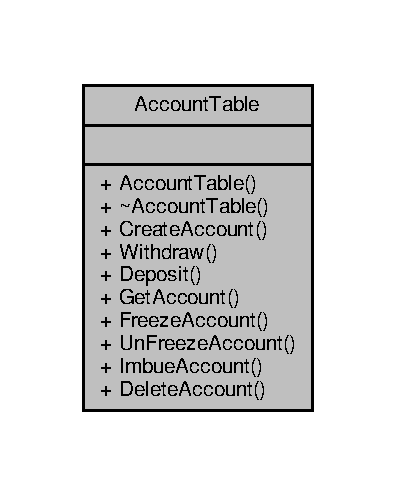
\includegraphics[width=190pt]{classAccountTable__coll__graph}
\end{center}
\end{figure}
\subsection*{Static Public Member Functions}
\begin{DoxyCompactItemize}
\item 
static long \hyperlink{classAccountTable_a21d33d81d195d65345eb0e62bfefcc25}{Create\-Account} (\hyperlink{classUser_1_1User}{User\-::\-User} \&user, long const \&account\-\_\-type)
\begin{DoxyCompactList}\small\item\em Creates a savings or chequing account for a user. \end{DoxyCompactList}\item 
static long \hyperlink{classAccountTable_a55eedcfb00f5eb7791248c540093c11c}{Withdraw} (\hyperlink{classAccount}{Account} \&account, double amount)
\begin{DoxyCompactList}\small\item\em Subtracts an amount from the account balance. \end{DoxyCompactList}\item 
\hypertarget{classAccountTable_a263c5492a4363f8b6759aa352c6f1b98}{static long {\bfseries Deposit} (\hyperlink{classAccount}{Account} \&account, double amount)}\label{classAccountTable_a263c5492a4363f8b6759aa352c6f1b98}

\item 
\hypertarget{classAccountTable_af21d68cc9288a375318ce48014dd3a97}{static long {\bfseries Get\-Account} (\hyperlink{classAccount}{Account} \&account, int \&id)}\label{classAccountTable_af21d68cc9288a375318ce48014dd3a97}

\item 
\hypertarget{classAccountTable_a607b08a95021ccf8f42871fe3f41fdef}{static long {\bfseries Freeze\-Account} (\hyperlink{classAccount}{Account} \&account)}\label{classAccountTable_a607b08a95021ccf8f42871fe3f41fdef}

\item 
\hypertarget{classAccountTable_a203e383ed970bc5275a3ed4ec8b0df9a}{static long {\bfseries Un\-Freeze\-Account} (\hyperlink{classAccount}{Account} \&account)}\label{classAccountTable_a203e383ed970bc5275a3ed4ec8b0df9a}

\item 
static long \hyperlink{classAccountTable_ab85511c89fe4be2c5862ea17815a672b}{Imbue\-Account} (std\-::vector$<$ std\-::string $>$ const \&column\-\_\-names, std\-::vector$<$ std\-::string $>$ row, \hyperlink{classAccount}{Account} \&account)
\begin{DoxyCompactList}\small\item\em Fills a the fields of an \hyperlink{classAccount}{Account} object from a row representing the account. \end{DoxyCompactList}\item 
static long \hyperlink{classAccountTable_a3ac0fd956589e65a005f225752adba32}{Delete\-Account} (\hyperlink{classAccount}{Account} \&account)
\begin{DoxyCompactList}\small\item\em Deletes an account from the database. \end{DoxyCompactList}\end{DoxyCompactItemize}


\subsection{Member Function Documentation}
\hypertarget{classAccountTable_a21d33d81d195d65345eb0e62bfefcc25}{\index{Account\-Table@{Account\-Table}!Create\-Account@{Create\-Account}}
\index{Create\-Account@{Create\-Account}!AccountTable@{Account\-Table}}
\subsubsection[{Create\-Account}]{\setlength{\rightskip}{0pt plus 5cm}long Account\-Table\-::\-Create\-Account (
\begin{DoxyParamCaption}
\item[{{\bf User\-::\-User} \&}]{user, }
\item[{long const \&}]{account\-\_\-type}
\end{DoxyParamCaption}
)\hspace{0.3cm}{\ttfamily [static]}}}\label{classAccountTable_a21d33d81d195d65345eb0e62bfefcc25}


Creates a savings or chequing account for a user. 


\begin{DoxyParams}{Parameters}
{\em user} & the user for whom to open the account \\
\hline
{\em account} & out parameter for the account \\
\hline
\end{DoxyParams}
\hypertarget{classAccountTable_a3ac0fd956589e65a005f225752adba32}{\index{Account\-Table@{Account\-Table}!Delete\-Account@{Delete\-Account}}
\index{Delete\-Account@{Delete\-Account}!AccountTable@{Account\-Table}}
\subsubsection[{Delete\-Account}]{\setlength{\rightskip}{0pt plus 5cm}long Account\-Table\-::\-Delete\-Account (
\begin{DoxyParamCaption}
\item[{{\bf Account} \&}]{account}
\end{DoxyParamCaption}
)\hspace{0.3cm}{\ttfamily [static]}}}\label{classAccountTable_a3ac0fd956589e65a005f225752adba32}


Deletes an account from the database. 


\begin{DoxyParams}{Parameters}
{\em account} & the account to delete \\
\hline
\end{DoxyParams}
\hypertarget{classAccountTable_ab85511c89fe4be2c5862ea17815a672b}{\index{Account\-Table@{Account\-Table}!Imbue\-Account@{Imbue\-Account}}
\index{Imbue\-Account@{Imbue\-Account}!AccountTable@{Account\-Table}}
\subsubsection[{Imbue\-Account}]{\setlength{\rightskip}{0pt plus 5cm}long Account\-Table\-::\-Imbue\-Account (
\begin{DoxyParamCaption}
\item[{std\-::vector$<$ std\-::string $>$ const \&}]{column\-\_\-names, }
\item[{std\-::vector$<$ std\-::string $>$}]{row, }
\item[{{\bf Account} \&}]{account}
\end{DoxyParamCaption}
)\hspace{0.3cm}{\ttfamily [static]}}}\label{classAccountTable_ab85511c89fe4be2c5862ea17815a672b}


Fills a the fields of an \hyperlink{classAccount}{Account} object from a row representing the account. 


\begin{DoxyParams}{Parameters}
{\em column\-\_\-names} & a list of the column names, ordered respectively, for the rows container \\
\hline
{\em row} & a row containing the account fields selected from the database \\
\hline
{\em account} & an out parameter to represent the user \\
\hline
\end{DoxyParams}
\hypertarget{classAccountTable_a55eedcfb00f5eb7791248c540093c11c}{\index{Account\-Table@{Account\-Table}!Withdraw@{Withdraw}}
\index{Withdraw@{Withdraw}!AccountTable@{Account\-Table}}
\subsubsection[{Withdraw}]{\setlength{\rightskip}{0pt plus 5cm}long Account\-Table\-::\-Withdraw (
\begin{DoxyParamCaption}
\item[{{\bf Account} \&}]{account, }
\item[{double}]{amount}
\end{DoxyParamCaption}
)\hspace{0.3cm}{\ttfamily [static]}}}\label{classAccountTable_a55eedcfb00f5eb7791248c540093c11c}


Subtracts an amount from the account balance. 


\begin{DoxyParams}{Parameters}
{\em account} & \\
\hline
{\em amount} & \\
\hline
\end{DoxyParams}


The documentation for this class was generated from the following files\-:\begin{DoxyCompactItemize}
\item 
src/\-Account/accounttable.\-h\item 
src/\-Account/accounttable.\-cpp\end{DoxyCompactItemize}

\hypertarget{classChequingAccount}{\section{Chequing\-Account Class Reference}
\label{classChequingAccount}\index{Chequing\-Account@{Chequing\-Account}}
}


Inheritance diagram for Chequing\-Account\-:
\nopagebreak
\begin{figure}[H]
\begin{center}
\leavevmode
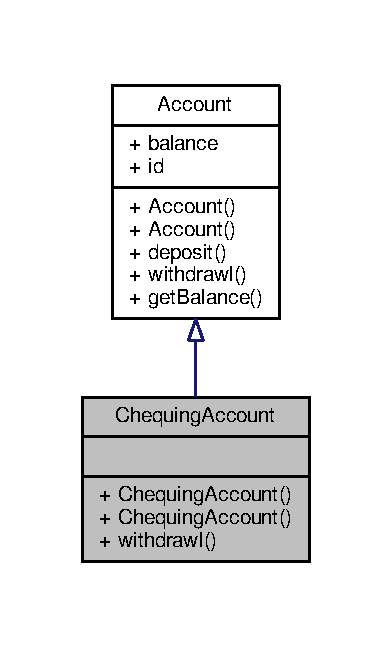
\includegraphics[width=188pt]{classChequingAccount__inherit__graph}
\end{center}
\end{figure}


Collaboration diagram for Chequing\-Account\-:
\nopagebreak
\begin{figure}[H]
\begin{center}
\leavevmode
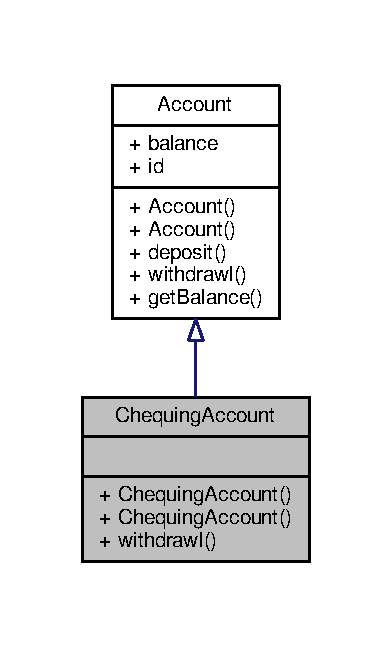
\includegraphics[width=188pt]{classChequingAccount__coll__graph}
\end{center}
\end{figure}
\subsection*{Public Member Functions}
\begin{DoxyCompactItemize}
\item 
\hyperlink{classChequingAccount_a865621271d561c98d980ebdb6001050d}{Chequing\-Account} (double balance)
\begin{DoxyCompactList}\small\item\em constructor that sets a starting balance \end{DoxyCompactList}\item 
\hyperlink{classChequingAccount_aaddd37c955dde9a6c18a733d14a887b2}{Chequing\-Account} ()
\begin{DoxyCompactList}\small\item\em default constructor. Balance is 0 \end{DoxyCompactList}\item 
virtual int \hyperlink{classChequingAccount_a58e0475e704c4bf69c671d6c2dc79a97}{withdrawl} (double amount)
\begin{DoxyCompactList}\small\item\em virtual method implementation of withdrawl \end{DoxyCompactList}\end{DoxyCompactItemize}
\subsection*{Additional Inherited Members}


\subsection{Constructor \& Destructor Documentation}
\hypertarget{classChequingAccount_a865621271d561c98d980ebdb6001050d}{\index{Chequing\-Account@{Chequing\-Account}!Chequing\-Account@{Chequing\-Account}}
\index{Chequing\-Account@{Chequing\-Account}!ChequingAccount@{Chequing\-Account}}
\subsubsection[{Chequing\-Account}]{\setlength{\rightskip}{0pt plus 5cm}Chequing\-Account\-::\-Chequing\-Account (
\begin{DoxyParamCaption}
\item[{double}]{balance}
\end{DoxyParamCaption}
)\hspace{0.3cm}{\ttfamily [inline]}}}\label{classChequingAccount_a865621271d561c98d980ebdb6001050d}


constructor that sets a starting balance 


\begin{DoxyParams}{Parameters}
{\em balance} & \\
\hline
\end{DoxyParams}
\hypertarget{classChequingAccount_aaddd37c955dde9a6c18a733d14a887b2}{\index{Chequing\-Account@{Chequing\-Account}!Chequing\-Account@{Chequing\-Account}}
\index{Chequing\-Account@{Chequing\-Account}!ChequingAccount@{Chequing\-Account}}
\subsubsection[{Chequing\-Account}]{\setlength{\rightskip}{0pt plus 5cm}Chequing\-Account\-::\-Chequing\-Account (
\begin{DoxyParamCaption}
{}
\end{DoxyParamCaption}
)\hspace{0.3cm}{\ttfamily [inline]}}}\label{classChequingAccount_aaddd37c955dde9a6c18a733d14a887b2}


default constructor. Balance is 0 



\subsection{Member Function Documentation}
\hypertarget{classChequingAccount_a58e0475e704c4bf69c671d6c2dc79a97}{\index{Chequing\-Account@{Chequing\-Account}!withdrawl@{withdrawl}}
\index{withdrawl@{withdrawl}!ChequingAccount@{Chequing\-Account}}
\subsubsection[{withdrawl}]{\setlength{\rightskip}{0pt plus 5cm}int Chequing\-Account\-::withdrawl (
\begin{DoxyParamCaption}
\item[{double}]{amount}
\end{DoxyParamCaption}
)\hspace{0.3cm}{\ttfamily [virtual]}}}\label{classChequingAccount_a58e0475e704c4bf69c671d6c2dc79a97}


virtual method implementation of withdrawl 


\begin{DoxyParams}{Parameters}
{\em amount} & to withdraw \\
\hline
\end{DoxyParams}
\begin{DoxyReturn}{Returns}
int 
\end{DoxyReturn}


Reimplemented from \hyperlink{classAccount_afe06e68bfc0e09eee1d39093c8f84704}{Account}.



The documentation for this class was generated from the following files\-:\begin{DoxyCompactItemize}
\item 
src/\-Account/chequingaccount.\-h\item 
src/\-Account/chequingaccount.\-cpp\end{DoxyCompactItemize}

\hypertarget{classCreditAccount}{\section{Credit\-Account Class Reference}
\label{classCreditAccount}\index{Credit\-Account@{Credit\-Account}}
}


Inheritance diagram for Credit\-Account\-:
\nopagebreak
\begin{figure}[H]
\begin{center}
\leavevmode
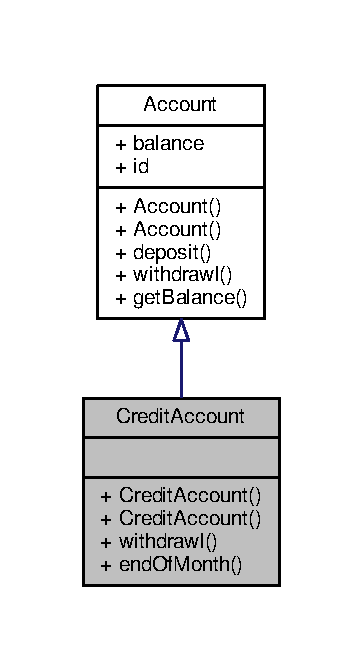
\includegraphics[width=174pt]{classCreditAccount__inherit__graph}
\end{center}
\end{figure}


Collaboration diagram for Credit\-Account\-:
\nopagebreak
\begin{figure}[H]
\begin{center}
\leavevmode
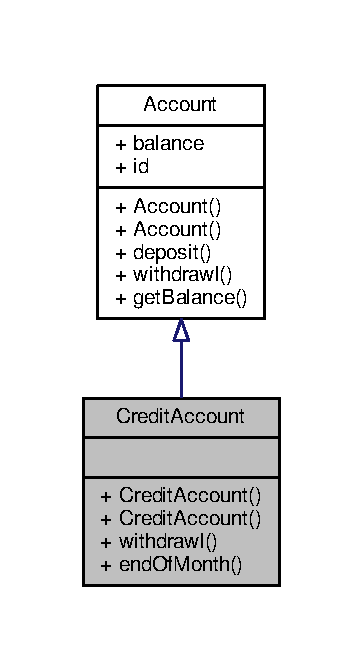
\includegraphics[width=174pt]{classCreditAccount__coll__graph}
\end{center}
\end{figure}
\subsection*{Public Member Functions}
\begin{DoxyCompactItemize}
\item 
\hypertarget{classCreditAccount_a7cb57eb14a18f97709071bc9150de1fe}{{\bfseries Credit\-Account} (double balance)}\label{classCreditAccount_a7cb57eb14a18f97709071bc9150de1fe}

\item 
virtual int \hyperlink{classCreditAccount_a56a3fd7d01d9767505895dbcec24ba4e}{withdrawl} (double amount)
\begin{DoxyCompactList}\small\item\em virtual method implementation of withdrawl \end{DoxyCompactList}\item 
void \hyperlink{classCreditAccount_a518d0efdb944a1d4233f70b4c97bd2cc}{end\-Of\-Month} ()
\begin{DoxyCompactList}\small\item\em performs end of month balances of credit account. \end{DoxyCompactList}\end{DoxyCompactItemize}
\subsection*{Additional Inherited Members}


\subsection{Member Function Documentation}
\hypertarget{classCreditAccount_a518d0efdb944a1d4233f70b4c97bd2cc}{\index{Credit\-Account@{Credit\-Account}!end\-Of\-Month@{end\-Of\-Month}}
\index{end\-Of\-Month@{end\-Of\-Month}!CreditAccount@{Credit\-Account}}
\subsubsection[{end\-Of\-Month}]{\setlength{\rightskip}{0pt plus 5cm}void Credit\-Account\-::end\-Of\-Month (
\begin{DoxyParamCaption}
{}
\end{DoxyParamCaption}
)}}\label{classCreditAccount_a518d0efdb944a1d4233f70b4c97bd2cc}


performs end of month balances of credit account. 

\hypertarget{classCreditAccount_a56a3fd7d01d9767505895dbcec24ba4e}{\index{Credit\-Account@{Credit\-Account}!withdrawl@{withdrawl}}
\index{withdrawl@{withdrawl}!CreditAccount@{Credit\-Account}}
\subsubsection[{withdrawl}]{\setlength{\rightskip}{0pt plus 5cm}int Credit\-Account\-::withdrawl (
\begin{DoxyParamCaption}
\item[{double}]{amount}
\end{DoxyParamCaption}
)\hspace{0.3cm}{\ttfamily [virtual]}}}\label{classCreditAccount_a56a3fd7d01d9767505895dbcec24ba4e}


virtual method implementation of withdrawl 


\begin{DoxyParams}{Parameters}
{\em amount} & of money to put onto credit card \\
\hline
\end{DoxyParams}
\begin{DoxyReturn}{Returns}
int 
\end{DoxyReturn}


Reimplemented from \hyperlink{classAccount_afe06e68bfc0e09eee1d39093c8f84704}{Account}.



The documentation for this class was generated from the following files\-:\begin{DoxyCompactItemize}
\item 
src/\-Account/creditaccount.\-h\item 
src/\-Account/creditaccount.\-cpp\end{DoxyCompactItemize}

\hypertarget{classDb_1_1Db}{\section{Db\-:\-:Db Class Reference}
\label{classDb_1_1Db}\index{Db\-::\-Db@{Db\-::\-Db}}
}


c++ class wrapper for a handful of static methods for accessing databases  




{\ttfamily \#include $<$db.\-h$>$}



Collaboration diagram for Db\-:\-:Db\-:
\nopagebreak
\begin{figure}[H]
\begin{center}
\leavevmode
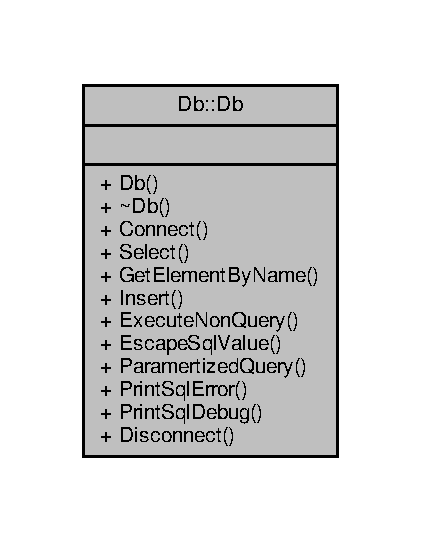
\includegraphics[width=202pt]{classDb_1_1Db__coll__graph}
\end{center}
\end{figure}
\subsection*{Static Public Member Functions}
\begin{DoxyCompactItemize}
\item 
static void \hyperlink{classDb_1_1Db_acb6baca594f012e54b3b413fc8490909}{Connect} ()
\begin{DoxyCompactList}\small\item\em Connects to the database. \end{DoxyCompactList}\item 
static long \hyperlink{classDb_1_1Db_a7adcafeb518814ae624e81bd998fe2c7}{Select} (std\-::string const \&query, \hyperlink{structDb_1_1db__rows}{db\-\_\-rows} \&rows)
\begin{DoxyCompactList}\small\item\em Performs a select query on the database and outputs \hyperlink{structDb_1_1db__rows}{db\-\_\-rows}. \end{DoxyCompactList}\item 
static std\-::string \hyperlink{classDb_1_1Db_a4a39f1b4090a66e07a9997c05291e857}{Get\-Element\-By\-Name} (std\-::string const \&name, std\-::vector$<$ std\-::string $>$ const \&column\-\_\-names, std\-::vector$<$ std\-::string $>$ const \&row)
\begin{DoxyCompactList}\small\item\em Gets an element of a row by its column name. \end{DoxyCompactList}\item 
static long \hyperlink{classDb_1_1Db_ade8f079023aa580603606d862afaba36}{Insert} (std\-::string const \&query, int \&id)
\begin{DoxyCompactList}\small\item\em Inserts a new row into the database and returns the id. \end{DoxyCompactList}\item 
static long \hyperlink{classDb_1_1Db_a7b7432985c8391482226a42a59e206fc}{Execute\-Non\-Query} (std\-::string const \&query, int \&rows\-\_\-affected)
\begin{DoxyCompactList}\small\item\em Executes a query on the database with the expectation that no result will be provided. \end{DoxyCompactList}\item 
static std\-::string \hyperlink{classDb_1_1Db_a6959db84448d62d069c761e3ce25d52c}{Escape\-Sql\-Value} (std\-::string const \&val)
\begin{DoxyCompactList}\small\item\em Escapes an S\-Q\-L value to thwart hackers. \end{DoxyCompactList}\item 
static std\-::string \hyperlink{classDb_1_1Db_acab38065a09648c66c53c1f948c48b6a}{Paramertized\-Query} (std\-::string query, std\-::vector$<$ std\-::string $>$ values)
\begin{DoxyCompactList}\small\item\em S\-Q\-L paramertized query. \end{DoxyCompactList}\item 
\hypertarget{classDb_1_1Db_a46c8f600cae71bddda3419a600e99136}{static void \hyperlink{classDb_1_1Db_a46c8f600cae71bddda3419a600e99136}{Print\-Sql\-Error} ()}\label{classDb_1_1Db_a46c8f600cae71bddda3419a600e99136}

\begin{DoxyCompactList}\small\item\em Prints all S\-Q\-L errors if S\-Q\-L\-\_\-\-P\-R\-I\-N\-T\-\_\-\-E\-R\-R\-O\-R\-S is defined. \end{DoxyCompactList}\item 
\hypertarget{classDb_1_1Db_ab0701e0bc17f6f01b0cbaaab05be3a6e}{static void \hyperlink{classDb_1_1Db_ab0701e0bc17f6f01b0cbaaab05be3a6e}{Print\-Sql\-Debug} (std\-::string const \&message)}\label{classDb_1_1Db_ab0701e0bc17f6f01b0cbaaab05be3a6e}

\begin{DoxyCompactList}\small\item\em Prints all S\-Q\-L debug messages if S\-Q\-L\-\_\-\-P\-R\-I\-N\-T\-\_\-\-D\-E\-B\-U\-G is defined. \end{DoxyCompactList}\item 
\hypertarget{classDb_1_1Db_a0f8b285970a00da958843ff27e05447b}{static void \hyperlink{classDb_1_1Db_a0f8b285970a00da958843ff27e05447b}{Disconnect} ()}\label{classDb_1_1Db_a0f8b285970a00da958843ff27e05447b}

\begin{DoxyCompactList}\small\item\em Disconnects from the database. \end{DoxyCompactList}\end{DoxyCompactItemize}


\subsection{Detailed Description}
c++ class wrapper for a handful of static methods for accessing databases 

Currently the only implemented database system is My\-S\-Q\-L 

\subsection{Member Function Documentation}
\hypertarget{classDb_1_1Db_acb6baca594f012e54b3b413fc8490909}{\index{Db\-::\-Db@{Db\-::\-Db}!Connect@{Connect}}
\index{Connect@{Connect}!Db::Db@{Db\-::\-Db}}
\subsubsection[{Connect}]{\setlength{\rightskip}{0pt plus 5cm}void Db\-::\-Db\-::\-Connect (
\begin{DoxyParamCaption}
{}
\end{DoxyParamCaption}
)\hspace{0.3cm}{\ttfamily [static]}}}\label{classDb_1_1Db_acb6baca594f012e54b3b413fc8490909}


Connects to the database. 


\begin{DoxyExceptions}{Exceptions}
{\em mysql} & error Makes a standard connection to the database and stores the result as a singleton object \\
\hline
\end{DoxyExceptions}
\hypertarget{classDb_1_1Db_a6959db84448d62d069c761e3ce25d52c}{\index{Db\-::\-Db@{Db\-::\-Db}!Escape\-Sql\-Value@{Escape\-Sql\-Value}}
\index{Escape\-Sql\-Value@{Escape\-Sql\-Value}!Db::Db@{Db\-::\-Db}}
\subsubsection[{Escape\-Sql\-Value}]{\setlength{\rightskip}{0pt plus 5cm}string Db\-::\-Db\-::\-Escape\-Sql\-Value (
\begin{DoxyParamCaption}
\item[{std\-::string const \&}]{val}
\end{DoxyParamCaption}
)\hspace{0.3cm}{\ttfamily [static]}}}\label{classDb_1_1Db_a6959db84448d62d069c761e3ce25d52c}


Escapes an S\-Q\-L value to thwart hackers. 


\begin{DoxyParams}{Parameters}
{\em val} & the string to be escaped \\
\hline
\end{DoxyParams}
\begin{DoxyReturn}{Returns}
a copy of the escaped string 
\end{DoxyReturn}
\hypertarget{classDb_1_1Db_a7b7432985c8391482226a42a59e206fc}{\index{Db\-::\-Db@{Db\-::\-Db}!Execute\-Non\-Query@{Execute\-Non\-Query}}
\index{Execute\-Non\-Query@{Execute\-Non\-Query}!Db::Db@{Db\-::\-Db}}
\subsubsection[{Execute\-Non\-Query}]{\setlength{\rightskip}{0pt plus 5cm}long Db\-::\-Db\-::\-Execute\-Non\-Query (
\begin{DoxyParamCaption}
\item[{std\-::string const \&}]{query, }
\item[{int \&}]{rows\-\_\-affected}
\end{DoxyParamCaption}
)\hspace{0.3cm}{\ttfamily [static]}}}\label{classDb_1_1Db_a7b7432985c8391482226a42a59e206fc}


Executes a query on the database with the expectation that no result will be provided. 


\begin{DoxyExceptions}{Exceptions}
{\em int} & S\-Q\-L\-\_\-\-Q\-U\-E\-R\-Y\-\_\-\-F\-A\-I\-L\-E\-D \\
\hline
\end{DoxyExceptions}

\begin{DoxyParams}{Parameters}
{\em query} & the A\-S\-C\-I\-I/utf8 S\-Q\-L statement \\
\hline
{\em rows\-\_\-affected} & out parameter representing the number of database rows affected by the query \\
\hline
\end{DoxyParams}
\hypertarget{classDb_1_1Db_a4a39f1b4090a66e07a9997c05291e857}{\index{Db\-::\-Db@{Db\-::\-Db}!Get\-Element\-By\-Name@{Get\-Element\-By\-Name}}
\index{Get\-Element\-By\-Name@{Get\-Element\-By\-Name}!Db::Db@{Db\-::\-Db}}
\subsubsection[{Get\-Element\-By\-Name}]{\setlength{\rightskip}{0pt plus 5cm}string Db\-::\-Db\-::\-Get\-Element\-By\-Name (
\begin{DoxyParamCaption}
\item[{std\-::string const \&}]{name, }
\item[{std\-::vector$<$ std\-::string $>$ const \&}]{column\-\_\-names, }
\item[{std\-::vector$<$ std\-::string $>$ const \&}]{row}
\end{DoxyParamCaption}
)\hspace{0.3cm}{\ttfamily [static]}}}\label{classDb_1_1Db_a4a39f1b4090a66e07a9997c05291e857}


Gets an element of a row by its column name. 


\begin{DoxyParams}{Parameters}
{\em name} & the name of the column \\
\hline
{\em column\-\_\-names} & a list of the column names, ordered respectively, for the rows container \\
\hline
{\em row} & the row of data selected from the table \\
\hline
\end{DoxyParams}
\begin{DoxyReturn}{Returns}
the value of the element in the same index position in the row container as the column name in the column\-\_\-names container 
\end{DoxyReturn}
\hypertarget{classDb_1_1Db_ade8f079023aa580603606d862afaba36}{\index{Db\-::\-Db@{Db\-::\-Db}!Insert@{Insert}}
\index{Insert@{Insert}!Db::Db@{Db\-::\-Db}}
\subsubsection[{Insert}]{\setlength{\rightskip}{0pt plus 5cm}long Db\-::\-Db\-::\-Insert (
\begin{DoxyParamCaption}
\item[{std\-::string const \&}]{query, }
\item[{int \&}]{id}
\end{DoxyParamCaption}
)\hspace{0.3cm}{\ttfamily [static]}}}\label{classDb_1_1Db_ade8f079023aa580603606d862afaba36}


Inserts a new row into the database and returns the id. 


\begin{DoxyParams}{Parameters}
{\em query} & the A\-S\-C\-I\-I/utf8 S\-Q\-L statement \\
\hline
{\em id} & output of the row id \\
\hline
\end{DoxyParams}
\hypertarget{classDb_1_1Db_acab38065a09648c66c53c1f948c48b6a}{\index{Db\-::\-Db@{Db\-::\-Db}!Paramertized\-Query@{Paramertized\-Query}}
\index{Paramertized\-Query@{Paramertized\-Query}!Db::Db@{Db\-::\-Db}}
\subsubsection[{Paramertized\-Query}]{\setlength{\rightskip}{0pt plus 5cm}std\-::string Db\-::\-Db\-::\-Paramertized\-Query (
\begin{DoxyParamCaption}
\item[{std\-::string}]{query, }
\item[{std\-::vector$<$ std\-::string $>$}]{values}
\end{DoxyParamCaption}
)\hspace{0.3cm}{\ttfamily [static]}}}\label{classDb_1_1Db_acab38065a09648c66c53c1f948c48b6a}


S\-Q\-L paramertized query. 

Emulates standard paramertized queries for database safety in preventing attacks.

Requires the same number of values as ? 
\begin{DoxyExceptions}{Exceptions}
{\em I\-N\-V\-A\-L\-I\-D\-\_\-\-P\-A\-R\-A\-M\-E\-R\-T\-I\-Z\-E\-D\-\_\-\-Q\-U\-E\-R\-Y} & \\
\hline
\end{DoxyExceptions}

\begin{DoxyParams}{Parameters}
{\em query} & the A\-S\-C\-I\-I/utf8 S\-Q\-L statement \\
\hline
{\em values} & the values that match the ?s to be replaced in the query \\
\hline
\end{DoxyParams}
\begin{DoxyReturn}{Returns}
a new string representing a safe S\-Q\-L query 
\end{DoxyReturn}
\hypertarget{classDb_1_1Db_a7adcafeb518814ae624e81bd998fe2c7}{\index{Db\-::\-Db@{Db\-::\-Db}!Select@{Select}}
\index{Select@{Select}!Db::Db@{Db\-::\-Db}}
\subsubsection[{Select}]{\setlength{\rightskip}{0pt plus 5cm}long Db\-::\-Db\-::\-Select (
\begin{DoxyParamCaption}
\item[{std\-::string const \&}]{query, }
\item[{{\bf db\-\_\-rows} \&}]{rows}
\end{DoxyParamCaption}
)\hspace{0.3cm}{\ttfamily [static]}}}\label{classDb_1_1Db_a7adcafeb518814ae624e81bd998fe2c7}


Performs a select query on the database and outputs \hyperlink{structDb_1_1db__rows}{db\-\_\-rows}. 

Runs a select and copies the memory to c++ containers and completes a \hyperlink{structDb_1_1db__rows}{db\-\_\-rows} struct 
\begin{DoxyExceptions}{Exceptions}
{\em int} & predefined database error constant \\
\hline
\end{DoxyExceptions}

\begin{DoxyParams}{Parameters}
{\em query} & the A\-S\-C\-I\-I/utf8 S\-Q\-L statement \\
\hline
{\em rows} & the result rows in c++ containers \\
\hline
\end{DoxyParams}


The documentation for this class was generated from the following files\-:\begin{DoxyCompactItemize}
\item 
src/\-Db/db.\-h\item 
src/\-Db/db.\-cpp\end{DoxyCompactItemize}

\hypertarget{structDb_1_1db__rows}{\section{Db\-:\-:db\-\_\-rows Struct Reference}
\label{structDb_1_1db__rows}\index{Db\-::db\-\_\-rows@{Db\-::db\-\_\-rows}}
}


A container for a set of rows.  




{\ttfamily \#include $<$db.\-h$>$}



Collaboration diagram for Db\-:\-:db\-\_\-rows\-:
\nopagebreak
\begin{figure}[H]
\begin{center}
\leavevmode
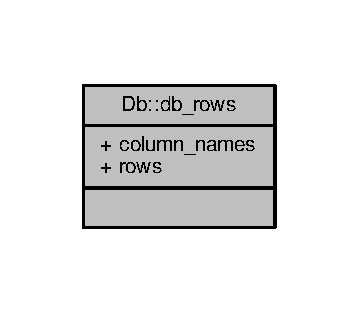
\includegraphics[width=172pt]{structDb_1_1db__rows__coll__graph}
\end{center}
\end{figure}
\subsection*{Public Attributes}
\begin{DoxyCompactItemize}
\item 
\hypertarget{structDb_1_1db__rows_ab5535960fe60a5b2e1a3c29883fb0828}{std\-::vector$<$ std\-::string $>$ {\bfseries column\-\_\-names}}\label{structDb_1_1db__rows_ab5535960fe60a5b2e1a3c29883fb0828}

\item 
\hypertarget{structDb_1_1db__rows_ad0e34a95070703cf4f46798b60ca2986}{std\-::vector$<$ std\-::vector\\*
$<$ std\-::string $>$ $>$ {\bfseries rows}}\label{structDb_1_1db__rows_ad0e34a95070703cf4f46798b60ca2986}

\end{DoxyCompactItemize}


\subsection{Detailed Description}
A container for a set of rows. 

Column names should be returned from all functions that return a set of rows, even if the set is 1 or 0 items in length The column\-\_\-name index will match the row column index for all rows in the set 

The documentation for this struct was generated from the following file\-:\begin{DoxyCompactItemize}
\item 
src/\-Db/db.\-h\end{DoxyCompactItemize}

\hypertarget{classFundMovementValidation}{\section{Fund\-Movement\-Validation Class Reference}
\label{classFundMovementValidation}\index{Fund\-Movement\-Validation@{Fund\-Movement\-Validation}}
}


Collaboration diagram for Fund\-Movement\-Validation\-:
\nopagebreak
\begin{figure}[H]
\begin{center}
\leavevmode
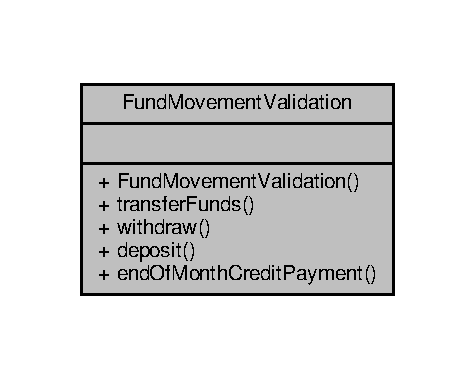
\includegraphics[width=228pt]{classFundMovementValidation__coll__graph}
\end{center}
\end{figure}
\subsection*{Public Member Functions}
\begin{DoxyCompactItemize}
\item 
\hyperlink{classFundMovementValidation_a77f3ec4e2f10391db28c8ab4ade75332}{Fund\-Movement\-Validation} ()
\begin{DoxyCompactList}\small\item\em default constructor \end{DoxyCompactList}\end{DoxyCompactItemize}
\subsection*{Static Public Member Functions}
\begin{DoxyCompactItemize}
\item 
static int \hyperlink{classFundMovementValidation_ad9e5d261bef007905722bac87e1f95c9}{transfer\-Funds} (\hyperlink{classAccount}{Account} \&from\-Account, \hyperlink{classAccount}{Account} \&to\-Account, double amount)
\begin{DoxyCompactList}\small\item\em Transfers funds from one account to another. \end{DoxyCompactList}\item 
static int \hyperlink{classFundMovementValidation_a4b9eddfeb255177cf5c45445a32e3e58}{withdraw} (\hyperlink{classAccount}{Account} \&from\-Account, double amount)
\begin{DoxyCompactList}\small\item\em withdraws money from an account \end{DoxyCompactList}\item 
static int \hyperlink{classFundMovementValidation_a9aebd2d98388d6c856fde366f5310b10}{deposit} (\hyperlink{classAccount}{Account} \&to\-Account, double amount)
\begin{DoxyCompactList}\small\item\em deposits money to an account \end{DoxyCompactList}\item 
\hypertarget{classFundMovementValidation_ad47ff42a70e417dff2d036a0f5373a30}{static int {\bfseries end\-Of\-Month\-Credit\-Payment} (\hyperlink{classUser_1_1User}{User\-::\-User} \&user, \hyperlink{classAccount}{Account} \&chequing\-Account, \hyperlink{classAccount}{Account} \&credit\-Account, double amount)}\label{classFundMovementValidation_ad47ff42a70e417dff2d036a0f5373a30}

\end{DoxyCompactItemize}


\subsection{Constructor \& Destructor Documentation}
\hypertarget{classFundMovementValidation_a77f3ec4e2f10391db28c8ab4ade75332}{\index{Fund\-Movement\-Validation@{Fund\-Movement\-Validation}!Fund\-Movement\-Validation@{Fund\-Movement\-Validation}}
\index{Fund\-Movement\-Validation@{Fund\-Movement\-Validation}!FundMovementValidation@{Fund\-Movement\-Validation}}
\subsubsection[{Fund\-Movement\-Validation}]{\setlength{\rightskip}{0pt plus 5cm}Fund\-Movement\-Validation\-::\-Fund\-Movement\-Validation (
\begin{DoxyParamCaption}
{}
\end{DoxyParamCaption}
)\hspace{0.3cm}{\ttfamily [inline]}}}\label{classFundMovementValidation_a77f3ec4e2f10391db28c8ab4ade75332}


default constructor 



\subsection{Member Function Documentation}
\hypertarget{classFundMovementValidation_a9aebd2d98388d6c856fde366f5310b10}{\index{Fund\-Movement\-Validation@{Fund\-Movement\-Validation}!deposit@{deposit}}
\index{deposit@{deposit}!FundMovementValidation@{Fund\-Movement\-Validation}}
\subsubsection[{deposit}]{\setlength{\rightskip}{0pt plus 5cm}int Fund\-Movement\-Validation\-::deposit (
\begin{DoxyParamCaption}
\item[{{\bf Account} \&}]{to\-Account, }
\item[{double}]{amount}
\end{DoxyParamCaption}
)\hspace{0.3cm}{\ttfamily [static]}}}\label{classFundMovementValidation_a9aebd2d98388d6c856fde366f5310b10}


deposits money to an account 


\begin{DoxyParams}{Parameters}
{\em to\-Account} & \\
\hline
{\em amount} & \\
\hline
\end{DoxyParams}
\begin{DoxyReturn}{Returns}

\end{DoxyReturn}
\hypertarget{classFundMovementValidation_ad9e5d261bef007905722bac87e1f95c9}{\index{Fund\-Movement\-Validation@{Fund\-Movement\-Validation}!transfer\-Funds@{transfer\-Funds}}
\index{transfer\-Funds@{transfer\-Funds}!FundMovementValidation@{Fund\-Movement\-Validation}}
\subsubsection[{transfer\-Funds}]{\setlength{\rightskip}{0pt plus 5cm}int Fund\-Movement\-Validation\-::transfer\-Funds (
\begin{DoxyParamCaption}
\item[{{\bf Account} \&}]{from\-Account, }
\item[{{\bf Account} \&}]{to\-Account, }
\item[{double}]{amount}
\end{DoxyParamCaption}
)\hspace{0.3cm}{\ttfamily [static]}}}\label{classFundMovementValidation_ad9e5d261bef007905722bac87e1f95c9}


Transfers funds from one account to another. 


\begin{DoxyParams}{Parameters}
{\em from\-Account} & the account to withdraw from \\
\hline
{\em to\-Account} & the account to deposit to \\
\hline
{\em amount} & the amount to transfer \\
\hline
\end{DoxyParams}
\begin{DoxyReturn}{Returns}
int 
\end{DoxyReturn}
\hypertarget{classFundMovementValidation_a4b9eddfeb255177cf5c45445a32e3e58}{\index{Fund\-Movement\-Validation@{Fund\-Movement\-Validation}!withdraw@{withdraw}}
\index{withdraw@{withdraw}!FundMovementValidation@{Fund\-Movement\-Validation}}
\subsubsection[{withdraw}]{\setlength{\rightskip}{0pt plus 5cm}int Fund\-Movement\-Validation\-::withdraw (
\begin{DoxyParamCaption}
\item[{{\bf Account} \&}]{from\-Account, }
\item[{double}]{amount}
\end{DoxyParamCaption}
)\hspace{0.3cm}{\ttfamily [static]}}}\label{classFundMovementValidation_a4b9eddfeb255177cf5c45445a32e3e58}


withdraws money from an account 


\begin{DoxyParams}{Parameters}
{\em from\-Account} & \\
\hline
{\em amount} & \\
\hline
\end{DoxyParams}
\begin{DoxyReturn}{Returns}

\end{DoxyReturn}


The documentation for this class was generated from the following files\-:\begin{DoxyCompactItemize}
\item 
src/\-Account/fundmovementvalidation.\-h\item 
src/\-Account/fundmovementvalidation.\-cpp\end{DoxyCompactItemize}

\hypertarget{classLogger}{\section{Logger Class Reference}
\label{classLogger}\index{Logger@{Logger}}
}


Collaboration diagram for Logger\-:
\nopagebreak
\begin{figure}[H]
\begin{center}
\leavevmode
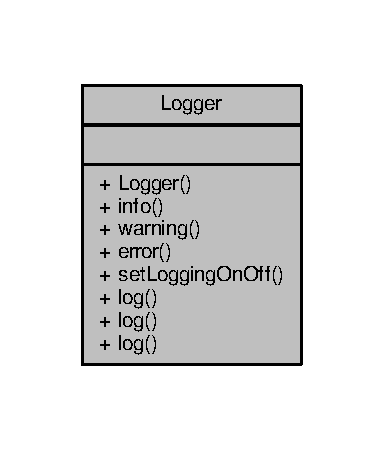
\includegraphics[width=184pt]{classLogger__coll__graph}
\end{center}
\end{figure}
\subsection*{Static Public Member Functions}
\begin{DoxyCompactItemize}
\item 
static void \hyperlink{classLogger_abd3c81f13327bf11d2523d2cadc5d34a}{info} (const string \&message)
\begin{DoxyCompactList}\small\item\em parameters are string -\/ the message to send to file \end{DoxyCompactList}\item 
static void \hyperlink{classLogger_ac4913cb3558a405491d8e01e254944a4}{warning} (const string \&message)
\begin{DoxyCompactList}\small\item\em parameters are string -\/ the message to send to file \end{DoxyCompactList}\item 
static void \hyperlink{classLogger_ade2e169a25c9fb5d0dc4b419b37566b3}{error} (const string \&message)
\begin{DoxyCompactList}\small\item\em parameters are string -\/ the message to send to file \end{DoxyCompactList}\item 
static void \hyperlink{classLogger_a5fcfe9604845c1fc90bdf4d8642e82c1}{set\-Logging\-On\-Off} (int on)
\begin{DoxyCompactList}\small\item\em parameters are string -\/ the message to send to file \end{DoxyCompactList}\item 
static void \hyperlink{classLogger_afd3da0948ec5bbea897b0f9d3379d7aa}{log} (int log\-Int, string \&user\-Name, double amount, const string \&account\-Type, const string \&from\-Account, const string \&to\-Account)
\begin{DoxyCompactList}\small\item\em used log\-Int to switch between multiple premade messages \end{DoxyCompactList}\item 
static void \hyperlink{classLogger_a65088a9394d167283dd7f3673c95c49d}{log} (int log\-Int, string \&user\-Name, double amount, const string \&account\-Type)
\begin{DoxyCompactList}\small\item\em uses log\-Int to switch between multiple premade messages \end{DoxyCompactList}\item 
static void \hyperlink{classLogger_a110813a074e05328bcc3be376a49b161}{log} (int log\-Int, string \&user\-Name)
\begin{DoxyCompactList}\small\item\em logs premade messages using log\-Int as the switch parameter \end{DoxyCompactList}\end{DoxyCompactItemize}


\subsection{Member Function Documentation}
\hypertarget{classLogger_ade2e169a25c9fb5d0dc4b419b37566b3}{\index{Logger@{Logger}!error@{error}}
\index{error@{error}!Logger@{Logger}}
\subsubsection[{error}]{\setlength{\rightskip}{0pt plus 5cm}void Logger\-::error (
\begin{DoxyParamCaption}
\item[{const string \&}]{message}
\end{DoxyParamCaption}
)\hspace{0.3cm}{\ttfamily [static]}}}\label{classLogger_ade2e169a25c9fb5d0dc4b419b37566b3}


parameters are string -\/ the message to send to file 


\begin{DoxyParams}{Parameters}
{\em message} & -\/ the message to print out as an error \\
\hline
\end{DoxyParams}
\hypertarget{classLogger_abd3c81f13327bf11d2523d2cadc5d34a}{\index{Logger@{Logger}!info@{info}}
\index{info@{info}!Logger@{Logger}}
\subsubsection[{info}]{\setlength{\rightskip}{0pt plus 5cm}void Logger\-::info (
\begin{DoxyParamCaption}
\item[{const string \&}]{message}
\end{DoxyParamCaption}
)\hspace{0.3cm}{\ttfamily [static]}}}\label{classLogger_abd3c81f13327bf11d2523d2cadc5d34a}


parameters are string -\/ the message to send to file 


\begin{DoxyParams}{Parameters}
{\em message} & the message to print as info \\
\hline
\end{DoxyParams}
\hypertarget{classLogger_afd3da0948ec5bbea897b0f9d3379d7aa}{\index{Logger@{Logger}!log@{log}}
\index{log@{log}!Logger@{Logger}}
\subsubsection[{log}]{\setlength{\rightskip}{0pt plus 5cm}void Logger\-::log (
\begin{DoxyParamCaption}
\item[{int}]{log\-Int, }
\item[{string \&}]{user\-Name, }
\item[{double}]{amount, }
\item[{const string \&}]{account\-Type, }
\item[{const string \&}]{from\-Account, }
\item[{const string \&}]{to\-Account}
\end{DoxyParamCaption}
)\hspace{0.3cm}{\ttfamily [static]}}}\label{classLogger_afd3da0948ec5bbea897b0f9d3379d7aa}


used log\-Int to switch between multiple premade messages 


\begin{DoxyParams}{Parameters}
{\em log\-Int} & the integer value -\/ defined in logger \\
\hline
{\em user\-Name} & -\/ username of the logged in user \\
\hline
{\em amount} & -\/ amount of money in this transaction \\
\hline
{\em account\-Type} & -\/ the account type in this transaction \\
\hline
{\em from\-Account} & -\/ the from account -\/ used for withdraws and transfers \\
\hline
{\em to\-Account} & -\/ the to account -\/ used for deposits and transfers \\
\hline
\end{DoxyParams}
\hypertarget{classLogger_a65088a9394d167283dd7f3673c95c49d}{\index{Logger@{Logger}!log@{log}}
\index{log@{log}!Logger@{Logger}}
\subsubsection[{log}]{\setlength{\rightskip}{0pt plus 5cm}void Logger\-::log (
\begin{DoxyParamCaption}
\item[{int}]{log\-Int, }
\item[{string \&}]{user\-Name, }
\item[{double}]{amount, }
\item[{const string \&}]{account\-Type}
\end{DoxyParamCaption}
)\hspace{0.3cm}{\ttfamily [static]}}}\label{classLogger_a65088a9394d167283dd7f3673c95c49d}


uses log\-Int to switch between multiple premade messages 


\begin{DoxyParams}{Parameters}
{\em log\-Int} & the interger value defined in logger \\
\hline
{\em user\-Name} & logged in user \\
\hline
{\em amount} & amount of money in transaction \\
\hline
{\em account\-Type} & the account type in the transaction \\
\hline
\end{DoxyParams}
\hypertarget{classLogger_a110813a074e05328bcc3be376a49b161}{\index{Logger@{Logger}!log@{log}}
\index{log@{log}!Logger@{Logger}}
\subsubsection[{log}]{\setlength{\rightskip}{0pt plus 5cm}void Logger\-::log (
\begin{DoxyParamCaption}
\item[{int}]{log\-Int, }
\item[{string \&}]{user\-Name}
\end{DoxyParamCaption}
)\hspace{0.3cm}{\ttfamily [static]}}}\label{classLogger_a110813a074e05328bcc3be376a49b161}


logs premade messages using log\-Int as the switch parameter 


\begin{DoxyParams}{Parameters}
{\em log\-Int} & defined in logger \\
\hline
{\em user\-Name} & user currently logged in \\
\hline
\end{DoxyParams}
\hypertarget{classLogger_a5fcfe9604845c1fc90bdf4d8642e82c1}{\index{Logger@{Logger}!set\-Logging\-On\-Off@{set\-Logging\-On\-Off}}
\index{set\-Logging\-On\-Off@{set\-Logging\-On\-Off}!Logger@{Logger}}
\subsubsection[{set\-Logging\-On\-Off}]{\setlength{\rightskip}{0pt plus 5cm}void Logger\-::set\-Logging\-On\-Off (
\begin{DoxyParamCaption}
\item[{int}]{on}
\end{DoxyParamCaption}
)\hspace{0.3cm}{\ttfamily [static]}}}\label{classLogger_a5fcfe9604845c1fc90bdf4d8642e82c1}


parameters are string -\/ the message to send to file 


\begin{DoxyParams}{Parameters}
{\em messagetakes} & an int 1 or 0 to turn on or off the logging\\
\hline
{\em on} & the int, 1 or 0, to turn on or off the logging \\
\hline
\end{DoxyParams}
\hypertarget{classLogger_ac4913cb3558a405491d8e01e254944a4}{\index{Logger@{Logger}!warning@{warning}}
\index{warning@{warning}!Logger@{Logger}}
\subsubsection[{warning}]{\setlength{\rightskip}{0pt plus 5cm}void Logger\-::warning (
\begin{DoxyParamCaption}
\item[{const string \&}]{message}
\end{DoxyParamCaption}
)\hspace{0.3cm}{\ttfamily [static]}}}\label{classLogger_ac4913cb3558a405491d8e01e254944a4}


parameters are string -\/ the message to send to file 


\begin{DoxyParams}{Parameters}
{\em message} & the message to print out as a warning \\
\hline
\end{DoxyParams}


The documentation for this class was generated from the following files\-:\begin{DoxyCompactItemize}
\item 
src/logger.\-h\item 
src/logger.\-cpp\end{DoxyCompactItemize}

\hypertarget{classMaintenanceMethods}{\section{Maintenance\-Methods Class Reference}
\label{classMaintenanceMethods}\index{Maintenance\-Methods@{Maintenance\-Methods}}
}


Collaboration diagram for Maintenance\-Methods\-:
\nopagebreak
\begin{figure}[H]
\begin{center}
\leavevmode
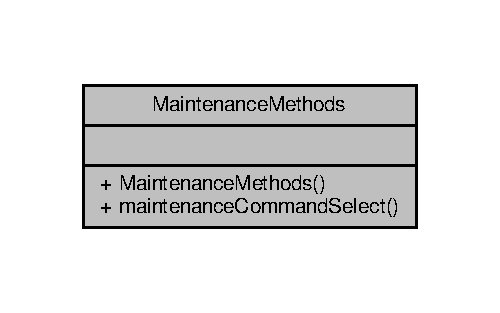
\includegraphics[width=240pt]{classMaintenanceMethods__coll__graph}
\end{center}
\end{figure}
\subsection*{Static Public Member Functions}
\begin{DoxyCompactItemize}
\item 
static void \hyperlink{classMaintenanceMethods_afb7690ca90af3ec170afe7d539baffca}{maintenance\-Command\-Select} (\hyperlink{classUser_1_1User}{User\-::\-User} \&user)
\begin{DoxyCompactList}\small\item\em the selection list for maintenance user \end{DoxyCompactList}\end{DoxyCompactItemize}


\subsection{Member Function Documentation}
\hypertarget{classMaintenanceMethods_afb7690ca90af3ec170afe7d539baffca}{\index{Maintenance\-Methods@{Maintenance\-Methods}!maintenance\-Command\-Select@{maintenance\-Command\-Select}}
\index{maintenance\-Command\-Select@{maintenance\-Command\-Select}!MaintenanceMethods@{Maintenance\-Methods}}
\subsubsection[{maintenance\-Command\-Select}]{\setlength{\rightskip}{0pt plus 5cm}void Maintenance\-Methods\-::maintenance\-Command\-Select (
\begin{DoxyParamCaption}
\item[{{\bf User\-::\-User} \&}]{user}
\end{DoxyParamCaption}
)\hspace{0.3cm}{\ttfamily [static]}}}\label{classMaintenanceMethods_afb7690ca90af3ec170afe7d539baffca}


the selection list for maintenance user 


\begin{DoxyParams}{Parameters}
{\em user} & passes user through \\
\hline
\end{DoxyParams}


The documentation for this class was generated from the following files\-:\begin{DoxyCompactItemize}
\item 
src/\-User/maintenancemethods.\-h\item 
src/\-User/maintenancemethods.\-cpp\end{DoxyCompactItemize}

\hypertarget{classManagerMethods}{\section{Manager\-Methods Class Reference}
\label{classManagerMethods}\index{Manager\-Methods@{Manager\-Methods}}
}


Collaboration diagram for Manager\-Methods\-:
\nopagebreak
\begin{figure}[H]
\begin{center}
\leavevmode
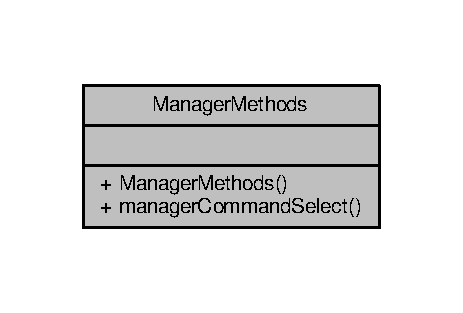
\includegraphics[width=222pt]{classManagerMethods__coll__graph}
\end{center}
\end{figure}
\subsection*{Static Public Member Functions}
\begin{DoxyCompactItemize}
\item 
static void \hyperlink{classManagerMethods_af2930adeae6a56e9615dace6c62331ee}{manager\-Command\-Select} (\hyperlink{classUser_1_1User}{User\-::\-User} \&user)
\begin{DoxyCompactList}\small\item\em allows manager user to select a list of commands \end{DoxyCompactList}\end{DoxyCompactItemize}


\subsection{Member Function Documentation}
\hypertarget{classManagerMethods_af2930adeae6a56e9615dace6c62331ee}{\index{Manager\-Methods@{Manager\-Methods}!manager\-Command\-Select@{manager\-Command\-Select}}
\index{manager\-Command\-Select@{manager\-Command\-Select}!ManagerMethods@{Manager\-Methods}}
\subsubsection[{manager\-Command\-Select}]{\setlength{\rightskip}{0pt plus 5cm}void Manager\-Methods\-::manager\-Command\-Select (
\begin{DoxyParamCaption}
\item[{{\bf User\-::\-User} \&}]{user}
\end{DoxyParamCaption}
)\hspace{0.3cm}{\ttfamily [static]}}}\label{classManagerMethods_af2930adeae6a56e9615dace6c62331ee}


allows manager user to select a list of commands 


\begin{DoxyParams}{Parameters}
{\em user} & \\
\hline
\end{DoxyParams}


The documentation for this class was generated from the following files\-:\begin{DoxyCompactItemize}
\item 
src/\-User/managermethods.\-h\item 
src/\-User/managermethods.\-cpp\end{DoxyCompactItemize}

\hypertarget{classPayment}{\section{Payment Class Reference}
\label{classPayment}\index{Payment@{Payment}}
}


Collaboration diagram for Payment\-:
\nopagebreak
\begin{figure}[H]
\begin{center}
\leavevmode
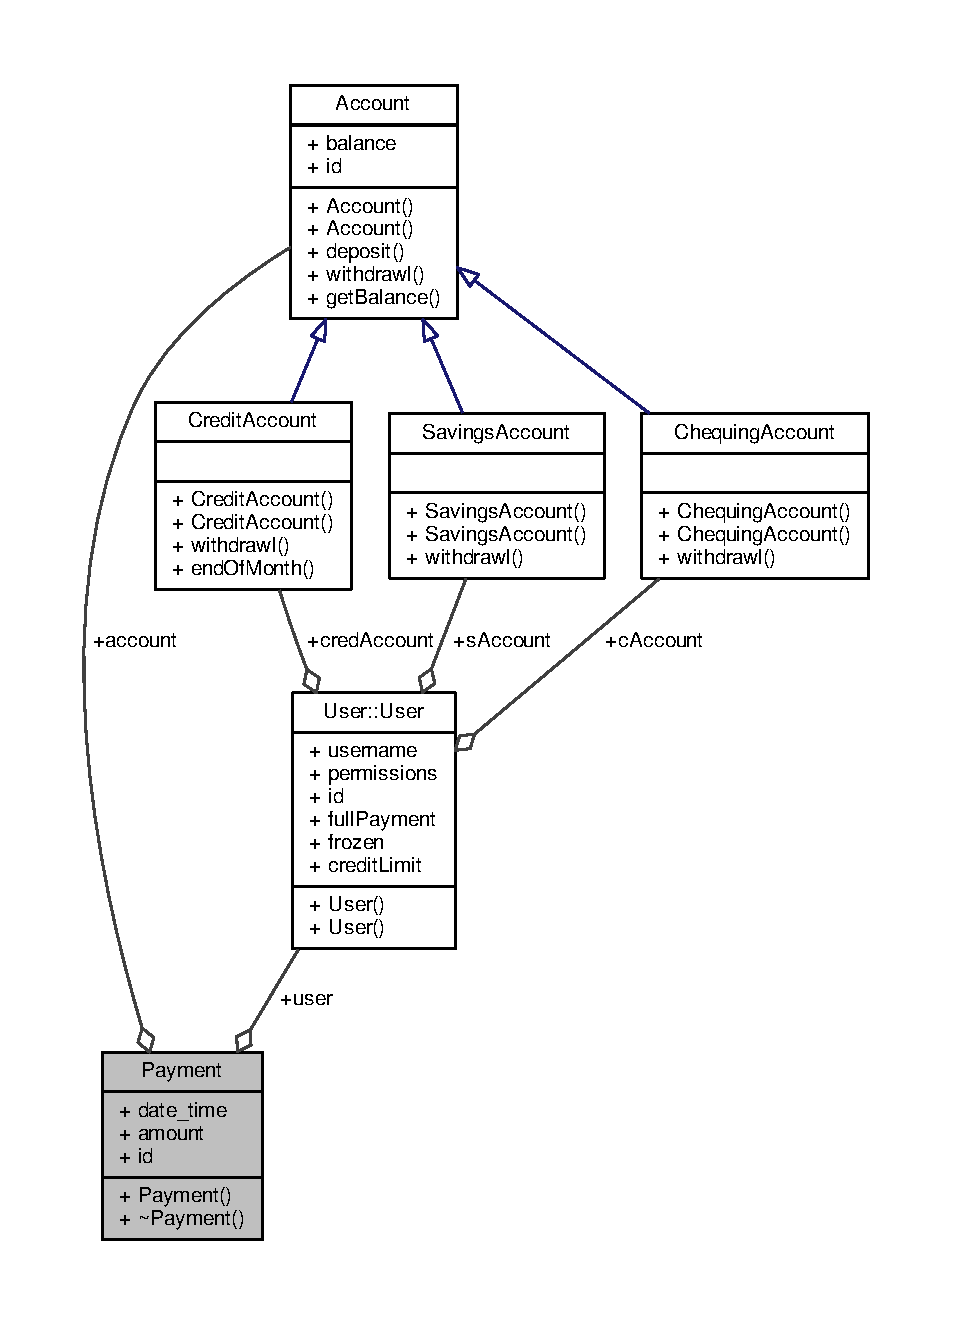
\includegraphics[width=350pt]{classPayment__coll__graph}
\end{center}
\end{figure}
\subsection*{Public Attributes}
\begin{DoxyCompactItemize}
\item 
\hypertarget{classPayment_aa902a90d3e2c6d0aba974738e015d810}{std\-::string {\bfseries date\-\_\-time}}\label{classPayment_aa902a90d3e2c6d0aba974738e015d810}

\item 
\hypertarget{classPayment_a6386cb08a31b3d4a9c9f3317a177502f}{int {\bfseries amount}}\label{classPayment_a6386cb08a31b3d4a9c9f3317a177502f}

\item 
\hypertarget{classPayment_afbfda92c58e679ff3613a2dc0f5e8d6e}{std\-::string {\bfseries id}}\label{classPayment_afbfda92c58e679ff3613a2dc0f5e8d6e}

\item 
\hypertarget{classPayment_a3cfe900556f61fdb630c9d0de54218c0}{\hyperlink{classAccount}{Account} {\bfseries account}}\label{classPayment_a3cfe900556f61fdb630c9d0de54218c0}

\item 
\hypertarget{classPayment_acf3f61dabeac253cd6a67a4c9e5c4832}{\hyperlink{classUser_1_1User}{User\-::\-User} {\bfseries user}}\label{classPayment_acf3f61dabeac253cd6a67a4c9e5c4832}

\end{DoxyCompactItemize}


The documentation for this class was generated from the following files\-:\begin{DoxyCompactItemize}
\item 
src/\-Payment/payment.\-h\item 
src/\-Payment/payment.\-cpp\end{DoxyCompactItemize}

\hypertarget{classPaymentTable}{\section{Payment\-Table Class Reference}
\label{classPaymentTable}\index{Payment\-Table@{Payment\-Table}}
}


Collaboration diagram for Payment\-Table\-:
\nopagebreak
\begin{figure}[H]
\begin{center}
\leavevmode
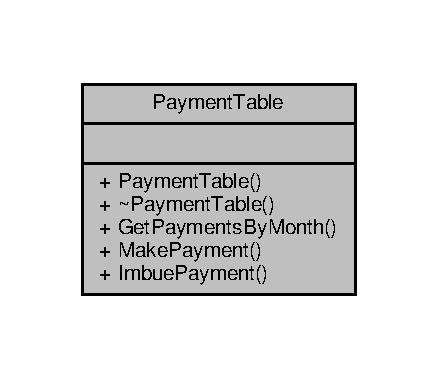
\includegraphics[width=210pt]{classPaymentTable__coll__graph}
\end{center}
\end{figure}
\subsection*{Static Public Member Functions}
\begin{DoxyCompactItemize}
\item 
\hypertarget{classPaymentTable_a8315ac37f00c78ba2e7d34af3b56ad9c}{static long {\bfseries Get\-Payments\-By\-Month} (int const \&year, int const \&month, \hyperlink{classAccount}{Account} const \&account, Payments \&payments)}\label{classPaymentTable_a8315ac37f00c78ba2e7d34af3b56ad9c}

\item 
\hypertarget{classPaymentTable_a935803f44af6e0c1437cfb9fb91b18f9}{static long {\bfseries Make\-Payment} (\hyperlink{classAccount}{Account} const \&account, int const \&amount)}\label{classPaymentTable_a935803f44af6e0c1437cfb9fb91b18f9}

\item 
\hypertarget{classPaymentTable_a73f9f69d18377f6bb395e1396eaefd2f}{static long {\bfseries Imbue\-Payment} (std\-::vector$<$ std\-::string $>$ const \&column\-\_\-names, std\-::vector$<$ std\-::string $>$ row, \hyperlink{classAccount}{Account} const \&account, \hyperlink{classPayment}{Payment} \&payment)}\label{classPaymentTable_a73f9f69d18377f6bb395e1396eaefd2f}

\end{DoxyCompactItemize}


The documentation for this class was generated from the following files\-:\begin{DoxyCompactItemize}
\item 
src/\-Payment/paymenttable.\-h\item 
src/\-Payment/paymenttable.\-cpp\end{DoxyCompactItemize}

\hypertarget{classPurchase}{\section{Purchase Class Reference}
\label{classPurchase}\index{Purchase@{Purchase}}
}


Collaboration diagram for Purchase\-:
\nopagebreak
\begin{figure}[H]
\begin{center}
\leavevmode
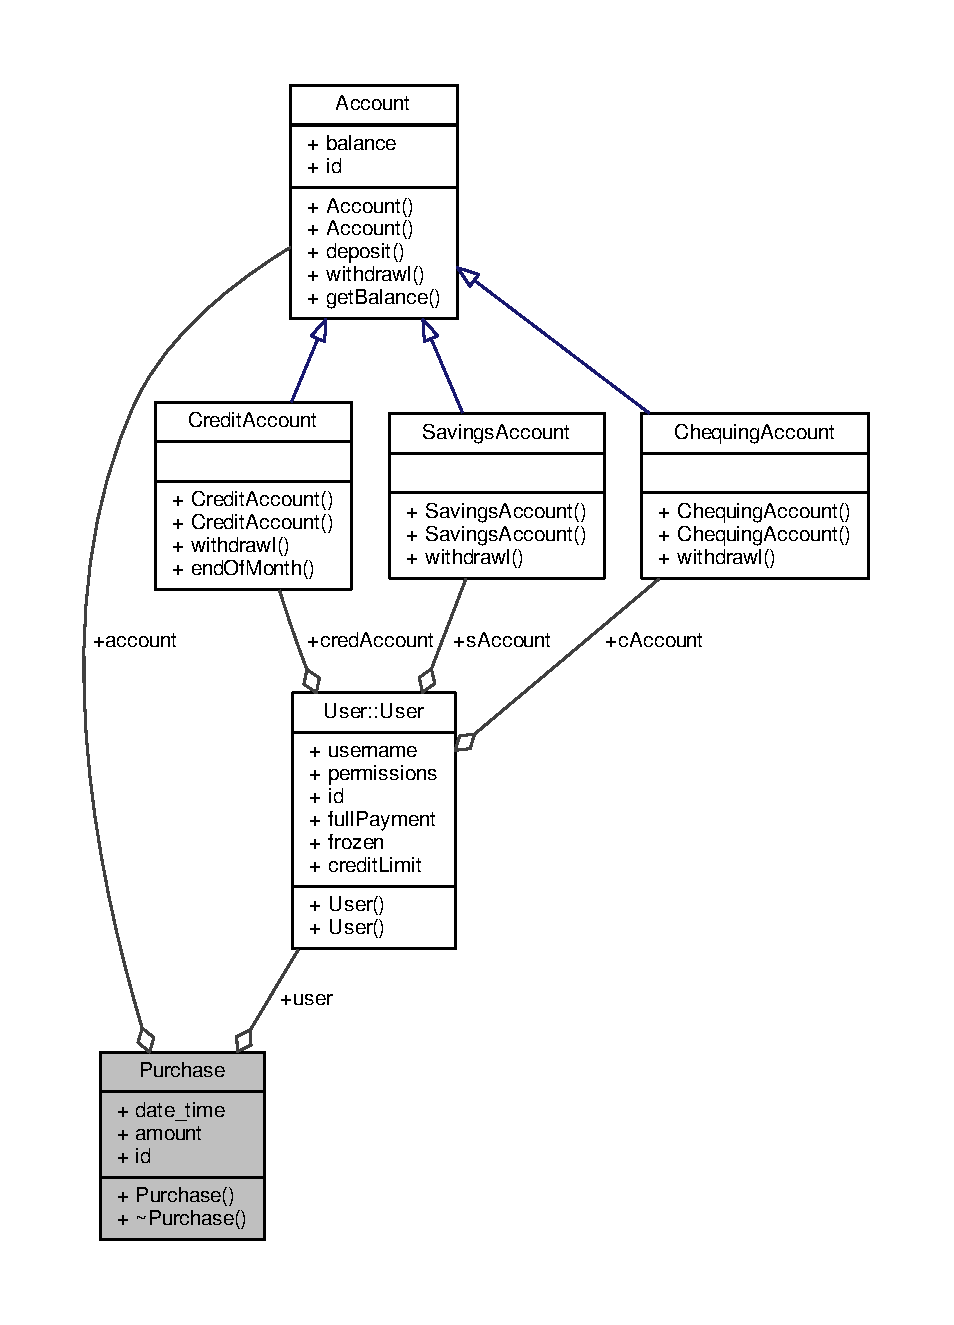
\includegraphics[width=350pt]{classPurchase__coll__graph}
\end{center}
\end{figure}
\subsection*{Public Attributes}
\begin{DoxyCompactItemize}
\item 
\hypertarget{classPurchase_acdb5fa722a3b86e08434bc08080299c4}{std\-::string {\bfseries date\-\_\-time}}\label{classPurchase_acdb5fa722a3b86e08434bc08080299c4}

\item 
\hypertarget{classPurchase_a8dc83cf3df8816ec75a71be285578c7e}{int {\bfseries amount}}\label{classPurchase_a8dc83cf3df8816ec75a71be285578c7e}

\item 
\hypertarget{classPurchase_aed492c0134dd3e746f4082f165bf1378}{std\-::string {\bfseries id}}\label{classPurchase_aed492c0134dd3e746f4082f165bf1378}

\item 
\hypertarget{classPurchase_a4572c7c8a290c4a916605349c4a53974}{\hyperlink{classAccount}{Account} {\bfseries account}}\label{classPurchase_a4572c7c8a290c4a916605349c4a53974}

\item 
\hypertarget{classPurchase_ae50d1aef59bd68dbc62a14d0fa72ff58}{\hyperlink{classUser_1_1User}{User\-::\-User} {\bfseries user}}\label{classPurchase_ae50d1aef59bd68dbc62a14d0fa72ff58}

\end{DoxyCompactItemize}


The documentation for this class was generated from the following files\-:\begin{DoxyCompactItemize}
\item 
src/\-Purchase/purchase.\-h\item 
src/\-Purchase/purchase.\-cpp\end{DoxyCompactItemize}

\hypertarget{classPurchaseTable}{\section{Purchase\-Table Class Reference}
\label{classPurchaseTable}\index{Purchase\-Table@{Purchase\-Table}}
}


Collaboration diagram for Purchase\-Table\-:
\nopagebreak
\begin{figure}[H]
\begin{center}
\leavevmode
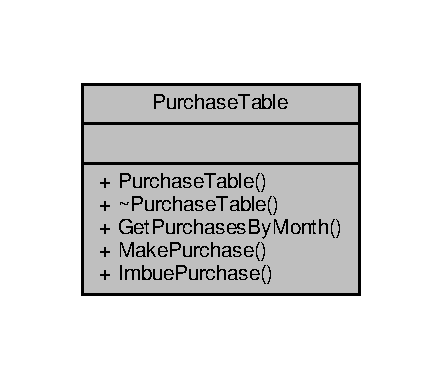
\includegraphics[width=212pt]{classPurchaseTable__coll__graph}
\end{center}
\end{figure}
\subsection*{Static Public Member Functions}
\begin{DoxyCompactItemize}
\item 
\hypertarget{classPurchaseTable_aba70ece26949ff6a10fb5f99268da681}{static long {\bfseries Get\-Purchases\-By\-Month} (int const \&year, int const \&month, \hyperlink{classAccount}{Account} const \&account, Purchases \&purchases)}\label{classPurchaseTable_aba70ece26949ff6a10fb5f99268da681}

\item 
\hypertarget{classPurchaseTable_a431e9fc9e6b017be67adc19e0dcb0eb2}{static long {\bfseries Make\-Purchase} (\hyperlink{classAccount}{Account} const \&account, int const \&amount)}\label{classPurchaseTable_a431e9fc9e6b017be67adc19e0dcb0eb2}

\item 
\hypertarget{classPurchaseTable_aca8b752313fbbf0a6143246f598078df}{static long {\bfseries Imbue\-Purchase} (std\-::vector$<$ std\-::string $>$ const \&column\-\_\-names, std\-::vector$<$ std\-::string $>$ row, \hyperlink{classAccount}{Account} const \&account, \hyperlink{classPurchase}{Purchase} \&purchase)}\label{classPurchaseTable_aca8b752313fbbf0a6143246f598078df}

\end{DoxyCompactItemize}


The documentation for this class was generated from the following files\-:\begin{DoxyCompactItemize}
\item 
src/\-Purchase/purchasetable.\-h\item 
src/\-Purchase/purchasetable.\-cpp\end{DoxyCompactItemize}

\hypertarget{classSavingsAccount}{\section{Savings\-Account Class Reference}
\label{classSavingsAccount}\index{Savings\-Account@{Savings\-Account}}
}


Inheritance diagram for Savings\-Account\-:
\nopagebreak
\begin{figure}[H]
\begin{center}
\leavevmode
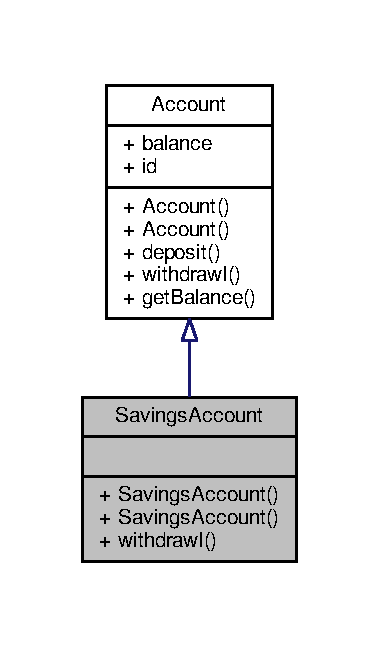
\includegraphics[width=182pt]{classSavingsAccount__inherit__graph}
\end{center}
\end{figure}


Collaboration diagram for Savings\-Account\-:
\nopagebreak
\begin{figure}[H]
\begin{center}
\leavevmode
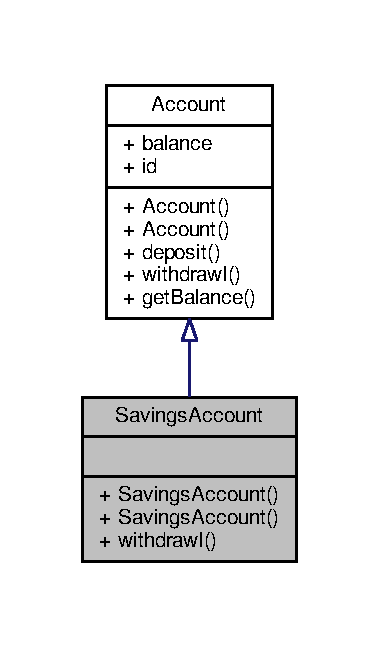
\includegraphics[width=182pt]{classSavingsAccount__coll__graph}
\end{center}
\end{figure}
\subsection*{Public Member Functions}
\begin{DoxyCompactItemize}
\item 
\hyperlink{classSavingsAccount_a6a1327106c71ba6e321d6b7c87bee117}{Savings\-Account} (double balance)
\begin{DoxyCompactList}\small\item\em constructor with starting balance \end{DoxyCompactList}\item 
\hyperlink{classSavingsAccount_ac4f23706b4f8fb55b7c898a974079ce5}{Savings\-Account} ()
\begin{DoxyCompactList}\small\item\em default constructor. Sets balance to0 \end{DoxyCompactList}\item 
virtual int \hyperlink{classSavingsAccount_ab79e02d7fd76e19a8b852eff489210df}{withdrawl} (double amount)
\begin{DoxyCompactList}\small\item\em virtual method implementation. \end{DoxyCompactList}\end{DoxyCompactItemize}
\subsection*{Additional Inherited Members}


\subsection{Constructor \& Destructor Documentation}
\hypertarget{classSavingsAccount_a6a1327106c71ba6e321d6b7c87bee117}{\index{Savings\-Account@{Savings\-Account}!Savings\-Account@{Savings\-Account}}
\index{Savings\-Account@{Savings\-Account}!SavingsAccount@{Savings\-Account}}
\subsubsection[{Savings\-Account}]{\setlength{\rightskip}{0pt plus 5cm}Savings\-Account\-::\-Savings\-Account (
\begin{DoxyParamCaption}
\item[{double}]{balance}
\end{DoxyParamCaption}
)\hspace{0.3cm}{\ttfamily [inline]}}}\label{classSavingsAccount_a6a1327106c71ba6e321d6b7c87bee117}


constructor with starting balance 


\begin{DoxyParams}{Parameters}
{\em balance} & \\
\hline
\end{DoxyParams}
\hypertarget{classSavingsAccount_ac4f23706b4f8fb55b7c898a974079ce5}{\index{Savings\-Account@{Savings\-Account}!Savings\-Account@{Savings\-Account}}
\index{Savings\-Account@{Savings\-Account}!SavingsAccount@{Savings\-Account}}
\subsubsection[{Savings\-Account}]{\setlength{\rightskip}{0pt plus 5cm}Savings\-Account\-::\-Savings\-Account (
\begin{DoxyParamCaption}
{}
\end{DoxyParamCaption}
)\hspace{0.3cm}{\ttfamily [inline]}}}\label{classSavingsAccount_ac4f23706b4f8fb55b7c898a974079ce5}


default constructor. Sets balance to0 



\subsection{Member Function Documentation}
\hypertarget{classSavingsAccount_ab79e02d7fd76e19a8b852eff489210df}{\index{Savings\-Account@{Savings\-Account}!withdrawl@{withdrawl}}
\index{withdrawl@{withdrawl}!SavingsAccount@{Savings\-Account}}
\subsubsection[{withdrawl}]{\setlength{\rightskip}{0pt plus 5cm}int Savings\-Account\-::withdrawl (
\begin{DoxyParamCaption}
\item[{double}]{amount}
\end{DoxyParamCaption}
)\hspace{0.3cm}{\ttfamily [virtual]}}}\label{classSavingsAccount_ab79e02d7fd76e19a8b852eff489210df}


virtual method implementation. 


\begin{DoxyParams}{Parameters}
{\em amount} & \\
\hline
\end{DoxyParams}
\begin{DoxyReturn}{Returns}

\end{DoxyReturn}


Reimplemented from \hyperlink{classAccount_afe06e68bfc0e09eee1d39093c8f84704}{Account}.



The documentation for this class was generated from the following files\-:\begin{DoxyCompactItemize}
\item 
src/\-Account/savingsaccount.\-h\item 
src/\-Account/savingsaccount.\-cpp\end{DoxyCompactItemize}

\hypertarget{classUser_1_1User}{\section{User\-:\-:User Class Reference}
\label{classUser_1_1User}\index{User\-::\-User@{User\-::\-User}}
}


Collaboration diagram for User\-:\-:User\-:
\nopagebreak
\begin{figure}[H]
\begin{center}
\leavevmode
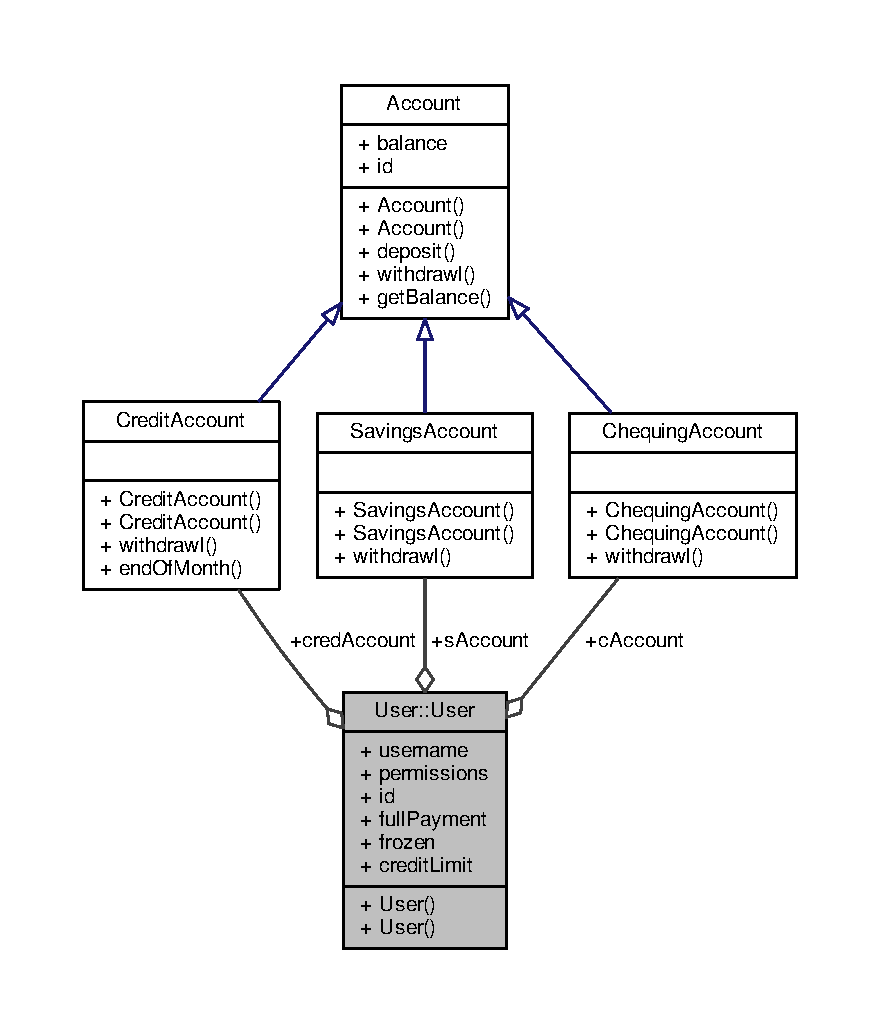
\includegraphics[width=350pt]{classUser_1_1User__coll__graph}
\end{center}
\end{figure}
\subsection*{Public Member Functions}
\begin{DoxyCompactItemize}
\item 
\hypertarget{classUser_1_1User_a8446d605c24cb948704c55b050b9bec8}{{\bfseries User} (std\-::string username)}\label{classUser_1_1User_a8446d605c24cb948704c55b050b9bec8}

\end{DoxyCompactItemize}
\subsection*{Public Attributes}
\begin{DoxyCompactItemize}
\item 
\hypertarget{classUser_1_1User_ac5858cf6e84e849b376862bf3b499702}{std\-::string {\bfseries username}}\label{classUser_1_1User_ac5858cf6e84e849b376862bf3b499702}

\item 
\hypertarget{classUser_1_1User_a3d945f509a0b28e0e5ed941b0d7b6a3a}{long {\bfseries permissions}}\label{classUser_1_1User_a3d945f509a0b28e0e5ed941b0d7b6a3a}

\item 
\hypertarget{classUser_1_1User_aa5cb0568ede3fa868173c2205f2d9296}{int {\bfseries id}}\label{classUser_1_1User_aa5cb0568ede3fa868173c2205f2d9296}

\item 
\hypertarget{classUser_1_1User_a3fb0c02b27de8a8593390ff476dd2483}{bool {\bfseries full\-Payment}}\label{classUser_1_1User_a3fb0c02b27de8a8593390ff476dd2483}

\item 
\hypertarget{classUser_1_1User_a1484e91101276d650e49c206730c2bb4}{\hyperlink{classChequingAccount}{Chequing\-Account} {\bfseries c\-Account}}\label{classUser_1_1User_a1484e91101276d650e49c206730c2bb4}

\item 
\hypertarget{classUser_1_1User_a2fb771418192be09c4458839ef097a52}{\hyperlink{classSavingsAccount}{Savings\-Account} {\bfseries s\-Account}}\label{classUser_1_1User_a2fb771418192be09c4458839ef097a52}

\item 
\hypertarget{classUser_1_1User_a51288924b7ef4375d13fbcc11ba62d20}{\hyperlink{classCreditAccount}{Credit\-Account} {\bfseries cred\-Account}}\label{classUser_1_1User_a51288924b7ef4375d13fbcc11ba62d20}

\item 
\hypertarget{classUser_1_1User_a1b23e9e4356623275c39fe437d501a83}{bool {\bfseries frozen}}\label{classUser_1_1User_a1b23e9e4356623275c39fe437d501a83}

\item 
\hypertarget{classUser_1_1User_abb60a21da252bfa75064d3b98dfc2b11}{int {\bfseries credit\-Limit}}\label{classUser_1_1User_abb60a21da252bfa75064d3b98dfc2b11}

\end{DoxyCompactItemize}


The documentation for this class was generated from the following files\-:\begin{DoxyCompactItemize}
\item 
src/\-User/user.\-h\item 
src/\-User/user.\-cpp\end{DoxyCompactItemize}

\hypertarget{classUserMethods}{\section{User\-Methods Class Reference}
\label{classUserMethods}\index{User\-Methods@{User\-Methods}}
}


Collaboration diagram for User\-Methods\-:
\nopagebreak
\begin{figure}[H]
\begin{center}
\leavevmode
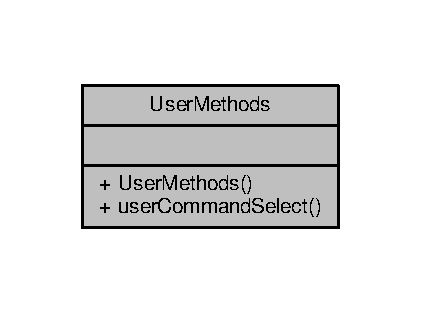
\includegraphics[width=202pt]{classUserMethods__coll__graph}
\end{center}
\end{figure}
\subsection*{Static Public Member Functions}
\begin{DoxyCompactItemize}
\item 
static void \hyperlink{classUserMethods_aa247ef5f63f1cb39d43bdb451d9ce1a7}{user\-Command\-Select} (\hyperlink{classUser_1_1User}{User\-::\-User} \&user)
\end{DoxyCompactItemize}


\subsection{Member Function Documentation}
\hypertarget{classUserMethods_aa247ef5f63f1cb39d43bdb451d9ce1a7}{\index{User\-Methods@{User\-Methods}!user\-Command\-Select@{user\-Command\-Select}}
\index{user\-Command\-Select@{user\-Command\-Select}!UserMethods@{User\-Methods}}
\subsubsection[{user\-Command\-Select}]{\setlength{\rightskip}{0pt plus 5cm}void User\-Methods\-::user\-Command\-Select (
\begin{DoxyParamCaption}
\item[{{\bf User\-::\-User} \&}]{user}
\end{DoxyParamCaption}
)\hspace{0.3cm}{\ttfamily [static]}}}\label{classUserMethods_aa247ef5f63f1cb39d43bdb451d9ce1a7}
brief allows user to select a command


\begin{DoxyParams}{Parameters}
{\em user} & \\
\hline
\end{DoxyParams}


The documentation for this class was generated from the following files\-:\begin{DoxyCompactItemize}
\item 
src/\-User/usermethods.\-h\item 
src/\-User/usermethods.\-cpp\end{DoxyCompactItemize}

\input{classusermethods}
\hypertarget{classUser_1_1UserTable}{\section{User\-:\-:User\-Table Class Reference}
\label{classUser_1_1UserTable}\index{User\-::\-User\-Table@{User\-::\-User\-Table}}
}


A list of static methods that access to the database for the \hyperlink{classUser_1_1User}{User} class.  




{\ttfamily \#include $<$usertable.\-h$>$}



Collaboration diagram for User\-:\-:User\-Table\-:
\nopagebreak
\begin{figure}[H]
\begin{center}
\leavevmode
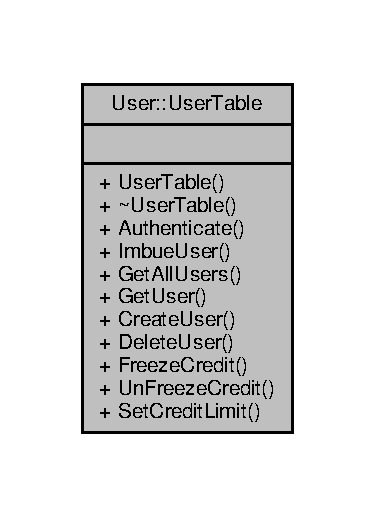
\includegraphics[width=180pt]{classUser_1_1UserTable__coll__graph}
\end{center}
\end{figure}
\subsection*{Static Public Member Functions}
\begin{DoxyCompactItemize}
\item 
static long \hyperlink{classUser_1_1UserTable_a805655228f47be97023baec681a2847e}{Authenticate} (std\-::string const \&username, std\-::string const \&password, \hyperlink{classUser_1_1User}{User} \&user)
\begin{DoxyCompactList}\small\item\em Compares a users credentials against the database and returns a \hyperlink{classUser_1_1User}{User} object if successful and throws an error otherwise. \end{DoxyCompactList}\item 
static long \hyperlink{classUser_1_1UserTable_a928ca6e6a4d8c2700280b3145e4df955}{Imbue\-User} (std\-::vector$<$ std\-::string $>$ const \&column\-\_\-names, std\-::vector$<$ std\-::string $>$ row, \hyperlink{classUser_1_1User}{User} \&user)
\begin{DoxyCompactList}\small\item\em Fills a the fields of a \hyperlink{classUser_1_1User}{User} object from a row representing the user. \end{DoxyCompactList}\item 
static long \hyperlink{classUser_1_1UserTable_a454047b50c369b81c9206f3d8e507a58}{Get\-All\-Users} (std\-::vector$<$ \hyperlink{classUser_1_1User}{User} $>$ \&users)
\begin{DoxyCompactList}\small\item\em Retrieves all users in the database for the admin. \end{DoxyCompactList}\item 
static long \hyperlink{classUser_1_1UserTable_ae258255d5d47944fbdaf87069dcbaace}{Get\-User} (std\-::string const \&username, \hyperlink{classUser_1_1User}{User} \&user)
\begin{DoxyCompactList}\small\item\em Retrieves a single user's information by username. \end{DoxyCompactList}\item 
static long \hyperlink{classUser_1_1UserTable_a5fd5bd887205ab0e59c366f20970891b}{Create\-User} (std\-::string const \&username, std\-::string const \&password, long permissions, bool full\-Payment, \hyperlink{classUser_1_1User}{User} \&user)
\begin{DoxyCompactList}\small\item\em Creates a user and adds it to the database. \end{DoxyCompactList}\item 
static long \hyperlink{classUser_1_1UserTable_a82ef3d56229c38733d9e0308fd772ba8}{Delete\-User} (std\-::string const \&username)
\begin{DoxyCompactList}\small\item\em Deletes a user from the database. \end{DoxyCompactList}\item 
\hypertarget{classUser_1_1UserTable_a4597d1a5ec8b748ad5fb761d5720dd07}{static long {\bfseries Freeze\-Credit} (\hyperlink{classUser_1_1User}{User} \&user)}\label{classUser_1_1UserTable_a4597d1a5ec8b748ad5fb761d5720dd07}

\item 
\hypertarget{classUser_1_1UserTable_ae79bc0a79ea8b4a1f43e5c6adda7adb6}{static long {\bfseries Un\-Freeze\-Credit} (\hyperlink{classUser_1_1User}{User} \&user)}\label{classUser_1_1UserTable_ae79bc0a79ea8b4a1f43e5c6adda7adb6}

\item 
\hypertarget{classUser_1_1UserTable_aad22cc215dfb8dcfbe379f2bccdbc175}{static long {\bfseries Set\-Credit\-Limit} (\hyperlink{classUser_1_1User}{User} \&user, int const \&credit\-\_\-limit)}\label{classUser_1_1UserTable_aad22cc215dfb8dcfbe379f2bccdbc175}

\end{DoxyCompactItemize}


\subsection{Detailed Description}
A list of static methods that access to the database for the \hyperlink{classUser_1_1User}{User} class. 

\subsection{Member Function Documentation}
\hypertarget{classUser_1_1UserTable_a805655228f47be97023baec681a2847e}{\index{User\-::\-User\-Table@{User\-::\-User\-Table}!Authenticate@{Authenticate}}
\index{Authenticate@{Authenticate}!User::UserTable@{User\-::\-User\-Table}}
\subsubsection[{Authenticate}]{\setlength{\rightskip}{0pt plus 5cm}long User\-::\-User\-Table\-::\-Authenticate (
\begin{DoxyParamCaption}
\item[{std\-::string const \&}]{username, }
\item[{std\-::string const \&}]{password, }
\item[{{\bf User} \&}]{user}
\end{DoxyParamCaption}
)\hspace{0.3cm}{\ttfamily [static]}}}\label{classUser_1_1UserTable_a805655228f47be97023baec681a2847e}


Compares a users credentials against the database and returns a \hyperlink{classUser_1_1User}{User} object if successful and throws an error otherwise. 


\begin{DoxyExceptions}{Exceptions}
{\em int} & A\-U\-T\-H\-E\-N\-T\-I\-C\-A\-T\-I\-O\-N\-\_\-\-F\-A\-I\-L\-U\-R\-E \\
\hline
\end{DoxyExceptions}

\begin{DoxyParams}{Parameters}
{\em username} & the username of the user to authenticate \\
\hline
{\em password} & the password of the user to authenticate \\
\hline
{\em user} & an out parameter to represent the user \\
\hline
\end{DoxyParams}
\hypertarget{classUser_1_1UserTable_a5fd5bd887205ab0e59c366f20970891b}{\index{User\-::\-User\-Table@{User\-::\-User\-Table}!Create\-User@{Create\-User}}
\index{Create\-User@{Create\-User}!User::UserTable@{User\-::\-User\-Table}}
\subsubsection[{Create\-User}]{\setlength{\rightskip}{0pt plus 5cm}long User\-::\-User\-Table\-::\-Create\-User (
\begin{DoxyParamCaption}
\item[{std\-::string const \&}]{username, }
\item[{std\-::string const \&}]{password, }
\item[{long}]{permissions, }
\item[{bool}]{full\-Payment, }
\item[{{\bf User} \&}]{user}
\end{DoxyParamCaption}
)\hspace{0.3cm}{\ttfamily [static]}}}\label{classUser_1_1UserTable_a5fd5bd887205ab0e59c366f20970891b}


Creates a user and adds it to the database. 


\begin{DoxyExceptions}{Exceptions}
{\em int} & C\-R\-E\-A\-T\-E\-\_\-\-U\-S\-E\-R\-\_\-\-F\-A\-I\-L\-U\-R\-E or C\-R\-E\-A\-T\-E\-\_\-\-U\-S\-E\-R\-\_\-\-F\-A\-I\-L\-U\-R\-E\-\_\-\-U\-S\-E\-R\-\_\-\-E\-X\-I\-S\-T\-S \\
\hline
\end{DoxyExceptions}

\begin{DoxyParams}{Parameters}
{\em username} & the user username \\
\hline
{\em password} & the user password \\
\hline
{\em permissions} & a bitwise value of the permissions based on the bit joining of permission constants \\
\hline
{\em user} & an out parameter to represent the user \\
\hline
\end{DoxyParams}
\hypertarget{classUser_1_1UserTable_a82ef3d56229c38733d9e0308fd772ba8}{\index{User\-::\-User\-Table@{User\-::\-User\-Table}!Delete\-User@{Delete\-User}}
\index{Delete\-User@{Delete\-User}!User::UserTable@{User\-::\-User\-Table}}
\subsubsection[{Delete\-User}]{\setlength{\rightskip}{0pt plus 5cm}long User\-::\-User\-Table\-::\-Delete\-User (
\begin{DoxyParamCaption}
\item[{std\-::string const \&}]{username}
\end{DoxyParamCaption}
)\hspace{0.3cm}{\ttfamily [static]}}}\label{classUser_1_1UserTable_a82ef3d56229c38733d9e0308fd772ba8}


Deletes a user from the database. 


\begin{DoxyExceptions}{Exceptions}
{\em int} & D\-E\-L\-E\-T\-E\-\_\-\-U\-S\-E\-R\-\_\-\-F\-A\-I\-L\-U\-R\-E \\
\hline
\end{DoxyExceptions}

\begin{DoxyParams}{Parameters}
{\em username} & the user username \\
\hline
\end{DoxyParams}
\hypertarget{classUser_1_1UserTable_a454047b50c369b81c9206f3d8e507a58}{\index{User\-::\-User\-Table@{User\-::\-User\-Table}!Get\-All\-Users@{Get\-All\-Users}}
\index{Get\-All\-Users@{Get\-All\-Users}!User::UserTable@{User\-::\-User\-Table}}
\subsubsection[{Get\-All\-Users}]{\setlength{\rightskip}{0pt plus 5cm}long User\-::\-User\-Table\-::\-Get\-All\-Users (
\begin{DoxyParamCaption}
\item[{std\-::vector$<$ {\bf User} $>$ \&}]{users}
\end{DoxyParamCaption}
)\hspace{0.3cm}{\ttfamily [static]}}}\label{classUser_1_1UserTable_a454047b50c369b81c9206f3d8e507a58}


Retrieves all users in the database for the admin. 


\begin{DoxyParams}{Parameters}
{\em users} & an out param for the users in the database \\
\hline
\end{DoxyParams}
\hypertarget{classUser_1_1UserTable_ae258255d5d47944fbdaf87069dcbaace}{\index{User\-::\-User\-Table@{User\-::\-User\-Table}!Get\-User@{Get\-User}}
\index{Get\-User@{Get\-User}!User::UserTable@{User\-::\-User\-Table}}
\subsubsection[{Get\-User}]{\setlength{\rightskip}{0pt plus 5cm}long User\-::\-User\-Table\-::\-Get\-User (
\begin{DoxyParamCaption}
\item[{std\-::string const \&}]{username, }
\item[{{\bf User} \&}]{user}
\end{DoxyParamCaption}
)\hspace{0.3cm}{\ttfamily [static]}}}\label{classUser_1_1UserTable_ae258255d5d47944fbdaf87069dcbaace}


Retrieves a single user's information by username. 


\begin{DoxyParams}{Parameters}
{\em username} & the username of the user to retrieve \\
\hline
{\em user} & the out param for the user \\
\hline
\end{DoxyParams}
\hypertarget{classUser_1_1UserTable_a928ca6e6a4d8c2700280b3145e4df955}{\index{User\-::\-User\-Table@{User\-::\-User\-Table}!Imbue\-User@{Imbue\-User}}
\index{Imbue\-User@{Imbue\-User}!User::UserTable@{User\-::\-User\-Table}}
\subsubsection[{Imbue\-User}]{\setlength{\rightskip}{0pt plus 5cm}long User\-::\-User\-Table\-::\-Imbue\-User (
\begin{DoxyParamCaption}
\item[{std\-::vector$<$ std\-::string $>$ const \&}]{column\-\_\-names, }
\item[{std\-::vector$<$ std\-::string $>$}]{row, }
\item[{{\bf User} \&}]{user}
\end{DoxyParamCaption}
)\hspace{0.3cm}{\ttfamily [static]}}}\label{classUser_1_1UserTable_a928ca6e6a4d8c2700280b3145e4df955}


Fills a the fields of a \hyperlink{classUser_1_1User}{User} object from a row representing the user. 


\begin{DoxyParams}{Parameters}
{\em column\-\_\-names} & a list of the column names, ordered respectively, for the rows container \\
\hline
{\em row} & a row containing the user fields selected from the database \\
\hline
{\em user} & an out parameter to represent the user \\
\hline
\end{DoxyParams}


The documentation for this class was generated from the following files\-:\begin{DoxyCompactItemize}
\item 
src/\-User/usertable.\-h\item 
src/\-User/usertable.\-cpp\end{DoxyCompactItemize}

\hypertarget{classUtilities}{\section{Utilities Class Reference}
\label{classUtilities}\index{Utilities@{Utilities}}
}


A wrapper class for general, repetitive tasks.  




{\ttfamily \#include $<$Utilities.\-h$>$}



Collaboration diagram for Utilities\-:
\nopagebreak
\begin{figure}[H]
\begin{center}
\leavevmode
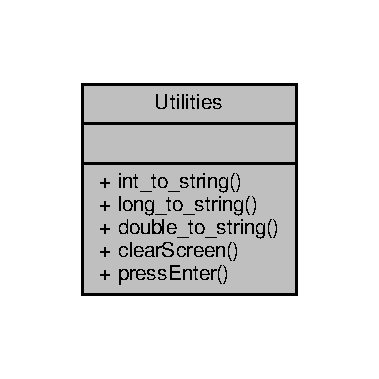
\includegraphics[width=182pt]{classUtilities__coll__graph}
\end{center}
\end{figure}
\subsection*{Static Public Member Functions}
\begin{DoxyCompactItemize}
\item 
static string \hyperlink{classUtilities_afc19dcfc998140c962a525e79c654d5a}{int\-\_\-to\-\_\-string} (int value)
\begin{DoxyCompactList}\small\item\em Converts an int to a string. \end{DoxyCompactList}\item 
static string \hyperlink{classUtilities_a67978e654e559751fb5ef62b650e28c3}{long\-\_\-to\-\_\-string} (long value)
\begin{DoxyCompactList}\small\item\em Converts a long to a string. \end{DoxyCompactList}\item 
static string \hyperlink{classUtilities_a4292e41b287aa5a64def0cf2268e6e43}{double\-\_\-to\-\_\-string} (double value)
\begin{DoxyCompactList}\small\item\em Converts a double to a string. \end{DoxyCompactList}\item 
\hypertarget{classUtilities_a480dcc8234bb28b9e8bf2f0e7109b620}{static void {\bfseries clear\-Screen} ()}\label{classUtilities_a480dcc8234bb28b9e8bf2f0e7109b620}

\item 
\hypertarget{classUtilities_a979e650bc17401e346d1db6744716cfb}{static void {\bfseries press\-Enter} ()}\label{classUtilities_a979e650bc17401e346d1db6744716cfb}

\end{DoxyCompactItemize}


\subsection{Detailed Description}
A wrapper class for general, repetitive tasks. 

\subsection{Member Function Documentation}
\hypertarget{classUtilities_a4292e41b287aa5a64def0cf2268e6e43}{\index{Utilities@{Utilities}!double\-\_\-to\-\_\-string@{double\-\_\-to\-\_\-string}}
\index{double\-\_\-to\-\_\-string@{double\-\_\-to\-\_\-string}!Utilities@{Utilities}}
\subsubsection[{double\-\_\-to\-\_\-string}]{\setlength{\rightskip}{0pt plus 5cm}static string Utilities\-::double\-\_\-to\-\_\-string (
\begin{DoxyParamCaption}
\item[{double}]{value}
\end{DoxyParamCaption}
)\hspace{0.3cm}{\ttfamily [inline]}, {\ttfamily [static]}}}\label{classUtilities_a4292e41b287aa5a64def0cf2268e6e43}


Converts a double to a string. 


\begin{DoxyParams}{Parameters}
{\em value} & the value to be converted \\
\hline
\end{DoxyParams}
\begin{DoxyReturn}{Returns}
a new string representing the converted value 
\end{DoxyReturn}
\hypertarget{classUtilities_afc19dcfc998140c962a525e79c654d5a}{\index{Utilities@{Utilities}!int\-\_\-to\-\_\-string@{int\-\_\-to\-\_\-string}}
\index{int\-\_\-to\-\_\-string@{int\-\_\-to\-\_\-string}!Utilities@{Utilities}}
\subsubsection[{int\-\_\-to\-\_\-string}]{\setlength{\rightskip}{0pt plus 5cm}static string Utilities\-::int\-\_\-to\-\_\-string (
\begin{DoxyParamCaption}
\item[{int}]{value}
\end{DoxyParamCaption}
)\hspace{0.3cm}{\ttfamily [inline]}, {\ttfamily [static]}}}\label{classUtilities_afc19dcfc998140c962a525e79c654d5a}


Converts an int to a string. 


\begin{DoxyParams}{Parameters}
{\em value} & the value to be converted \\
\hline
\end{DoxyParams}
\begin{DoxyReturn}{Returns}
a new string representing the converted value 
\end{DoxyReturn}
\hypertarget{classUtilities_a67978e654e559751fb5ef62b650e28c3}{\index{Utilities@{Utilities}!long\-\_\-to\-\_\-string@{long\-\_\-to\-\_\-string}}
\index{long\-\_\-to\-\_\-string@{long\-\_\-to\-\_\-string}!Utilities@{Utilities}}
\subsubsection[{long\-\_\-to\-\_\-string}]{\setlength{\rightskip}{0pt plus 5cm}static string Utilities\-::long\-\_\-to\-\_\-string (
\begin{DoxyParamCaption}
\item[{long}]{value}
\end{DoxyParamCaption}
)\hspace{0.3cm}{\ttfamily [inline]}, {\ttfamily [static]}}}\label{classUtilities_a67978e654e559751fb5ef62b650e28c3}


Converts a long to a string. 


\begin{DoxyParams}{Parameters}
{\em value} & the value to be converted \\
\hline
\end{DoxyParams}
\begin{DoxyReturn}{Returns}
a new string representing the converted value 
\end{DoxyReturn}


The documentation for this class was generated from the following file\-:\begin{DoxyCompactItemize}
\item 
src/Utilities.\-h\end{DoxyCompactItemize}

%--- End generated contents ---

% Index
\newpage
\phantomsection
\addcontentsline{toc}{chapter}{Index}
\printindex

\end{document}
